\documentclass[aspectratio=169,pdf]{beamer}

% Stanford theme
\usepackage{graphicx}
\usepackage{booktabs}
\usepackage{tikz}
\usetikzlibrary{patterns}
\usepackage{xcolor}
\usepackage{caption}
\captionsetup[figure]{labelformat=empty}
\usepackage{tcolorbox}
\graphicspath{{figures/}}

\usetheme{Stanford}
\input{./style_files_stanford/my_beamer_defs.sty}
\logo{
\includegraphics[height=0.4in]{./style_files_stanford/SU_New_BlockStree_2color.png}}

% Tighter margins for figures
\setbeamersize{text margin left=8mm, text margin right=8mm}

% Custom callout boxes using Stanford colors
\newcommand{\statbox}[1]{%
  \begin{tikzpicture}
    \node[fill=alertbg, draw=cardinalred, rounded corners=4pt, inner sep=6pt, line width=0.8pt] {%
      \color{cardinalred}\bfseries #1};
  \end{tikzpicture}%
}
\definecolor{alertbg}{RGB}{255,235,235}

\newcommand{\insightbox}[1]{%
  \begin{tikzpicture}
    \node[fill=insightbg, draw=darkcyan, rounded corners=4pt, inner sep=6pt, line width=0.8pt, text width=0.85\textwidth] {%
      \color{darkcyan}\bfseries #1};
  \end{tikzpicture}%
}
\definecolor{insightbg}{RGB}{230,245,255}

\newcommand{\empy}[1]{{\color{darkorange}\emph{#1}}}
\newcommand{\empr}[1]{{\color{cardinalred}\emph{#1}}}

% Title
\title[GPU Sched]{Pack Smart, Schedule Fair}
\subtitle{Unifying Heterogeneity and Fragmentation Awareness in GPU Scheduling}

\beamertemplatenavigationsymbolsempty

\begin{document}

\author[Stanford]{
	\begin{tabular}{c | c | c | c}
	Varun Ramesh & Jiayu Chang & Hyeonggyu Kim & Stefan Ene
\end{tabular}
\vspace{-4ex}}

\institute{
	
\includegraphics[height=0.4in]{./style_files_stanford/SU_New_BlockStree_2color.png}\\
	CS244C -- Advanced Topics in Networking\\
	Stanford University}

\date{Winter 2026}

% ============================================================
% TITLE SLIDE
% ============================================================
\begin{noheadline}
\begin{frame}\maketitle\end{frame}
\end{noheadline}

% ============================================================
% SLIDE 1: Problem -- Two Sources of Wasted GPU Capacity
% ============================================================
\begin{frame}{Two Problems Reduce Effective GPU Capacity}

\begin{center}
  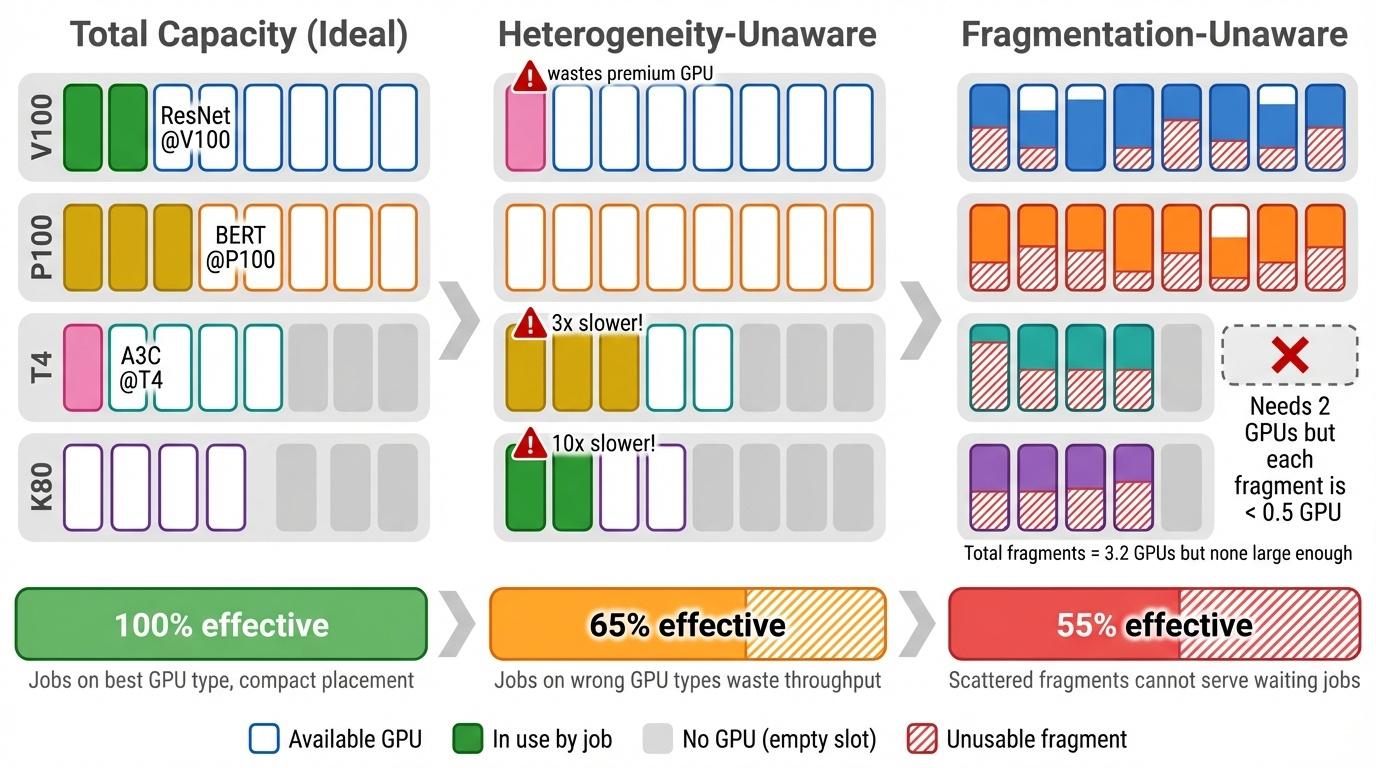
\includegraphics[width=\textwidth,height=0.85\textheight,keepaspectratio]{fig_slide1_capacity_v4.png}
\end{center}

\note{
  \begin{itemize}
    \item GPU clusters are expensive. Two problems erode effective capacity.
    \item LEFT: Ideal -- jobs on best GPU type, compact placement, 100\% effective.
    \item MIDDLE: Heterogeneity-unaware -- ResNet on K80 (10x slower!), BERT on T4 (3x slower!). 65\% effective.
    \item RIGHT: Fragmentation -- every GPU partially used, fragments too small for waiting jobs. 3.2 GPUs of fragments but none large enough. 55\% effective.
    \item TRANSITION: Two recent systems tackle one problem each...
  \end{itemize}
}

\end{frame}

% ============================================================
% SLIDE 2: Two Systems, One Gap
% ============================================================
\begin{frame}{Two Systems, One Gap}

\begin{columns}[T]
\begin{column}{0.44\textwidth}
  \centering
  \textbf{Gavel} \textit{(OSDI 2020)}\\[4pt]
  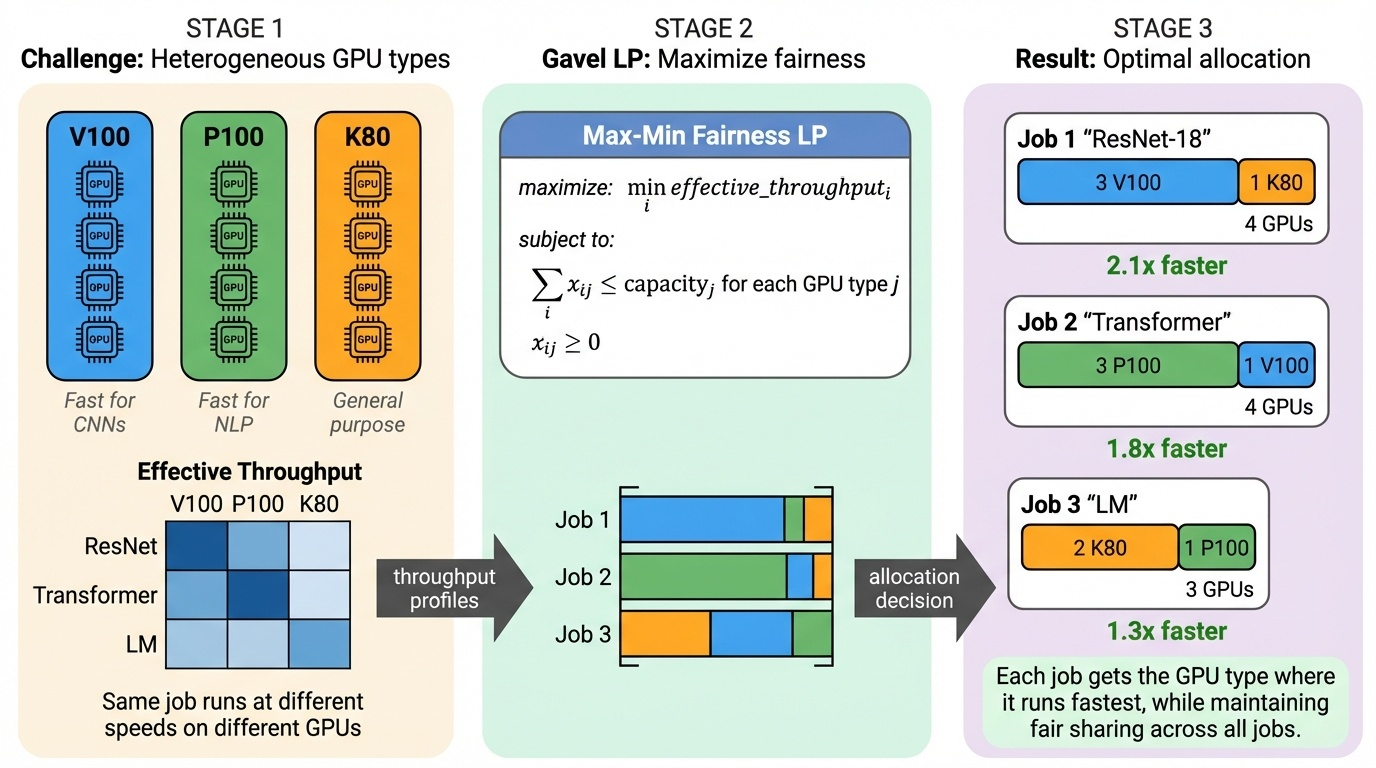
\includegraphics[width=0.95\textwidth]{fig2_gavel_algorithm.png}\\[4pt]
  \small Solves LP to allocate jobs across GPU types.\\
  Reduces JCT by 20--70\%.\\[6pt]
  \textcolor{cardinalred}{\textbf{Gap:} Ignores \textit{where} jobs land.}
\end{column}

\begin{column}{0.12\textwidth}
  \centering
  \vspace{2cm}
  \Large $+$\\[8pt]
  \normalsize \textcolor{gray}{?}
\end{column}

\begin{column}{0.44\textwidth}
  \centering
  \textbf{FGD} \textit{(ATC 2023)}\\[4pt]
  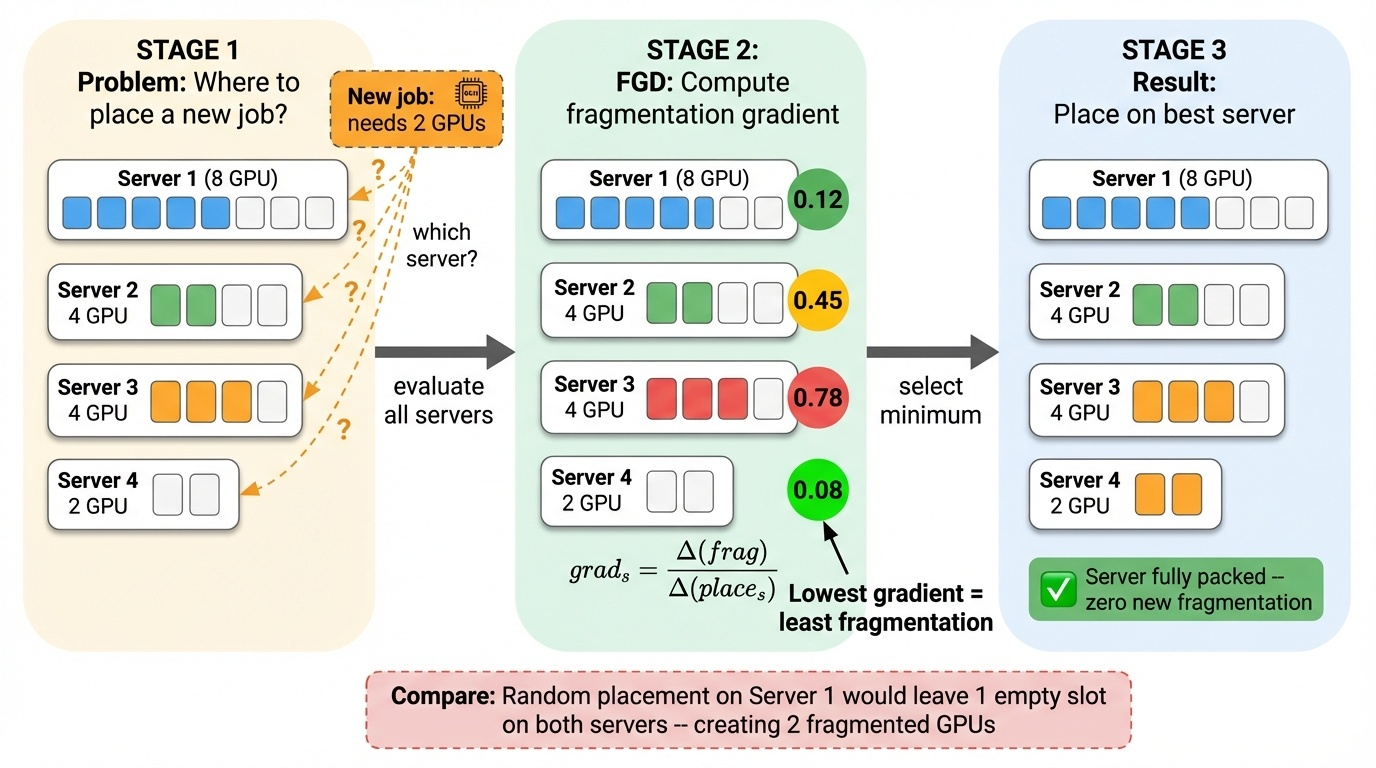
\includegraphics[width=0.95\textwidth]{fig3_fgd_algorithm.png}\\[4pt]
  \small Places jobs to minimize fragmentation gradient.\\
  Reduces wasted GPUs by 49\%.\\[6pt]
  \textcolor{cardinalred}{\textbf{Gap:} No flexible policy framework.}
\end{column}
\end{columns}

\note{
  \begin{itemize}
    \item Gavel solves an LP to allocate jobs across GPU types based on per-model throughput.
    \item FGD places each job on the node that minimizes fragmentation growth.
    \item They operate at different levels: Gavel picks WHICH GPU type, FGD picks WHICH node.
    \item Natural question: what if we combine them?
    \item TRANSITION: Our approach layers them...
  \end{itemize}
}

\end{frame}

% ============================================================
% SLIDE 3: Our Approach -- Context + Architecture
% ============================================================
\begin{frame}{Our Approach: Bridging Two Research Lines}

\begin{columns}[T]
\begin{column}{0.42\textwidth}
  \centering
  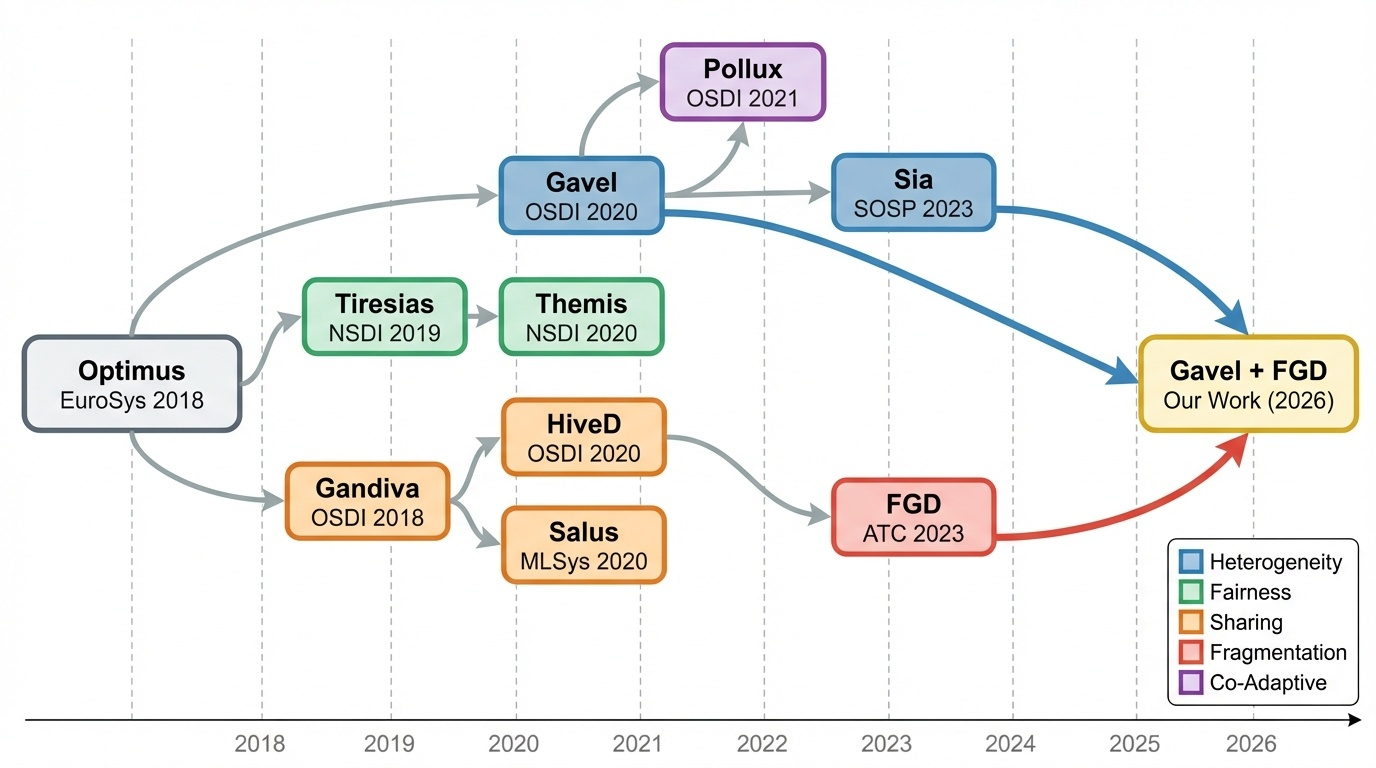
\includegraphics[width=\textwidth,height=0.55\textheight,keepaspectratio]{fig_literature_genealogy.png}\\[2pt]
  \footnotesize Research lineage: heterogeneity-aware (blue),\\fragmentation-aware (red). \textbf{Our work bridges both.}
\end{column}
\begin{column}{0.55\textwidth}
  \centering
  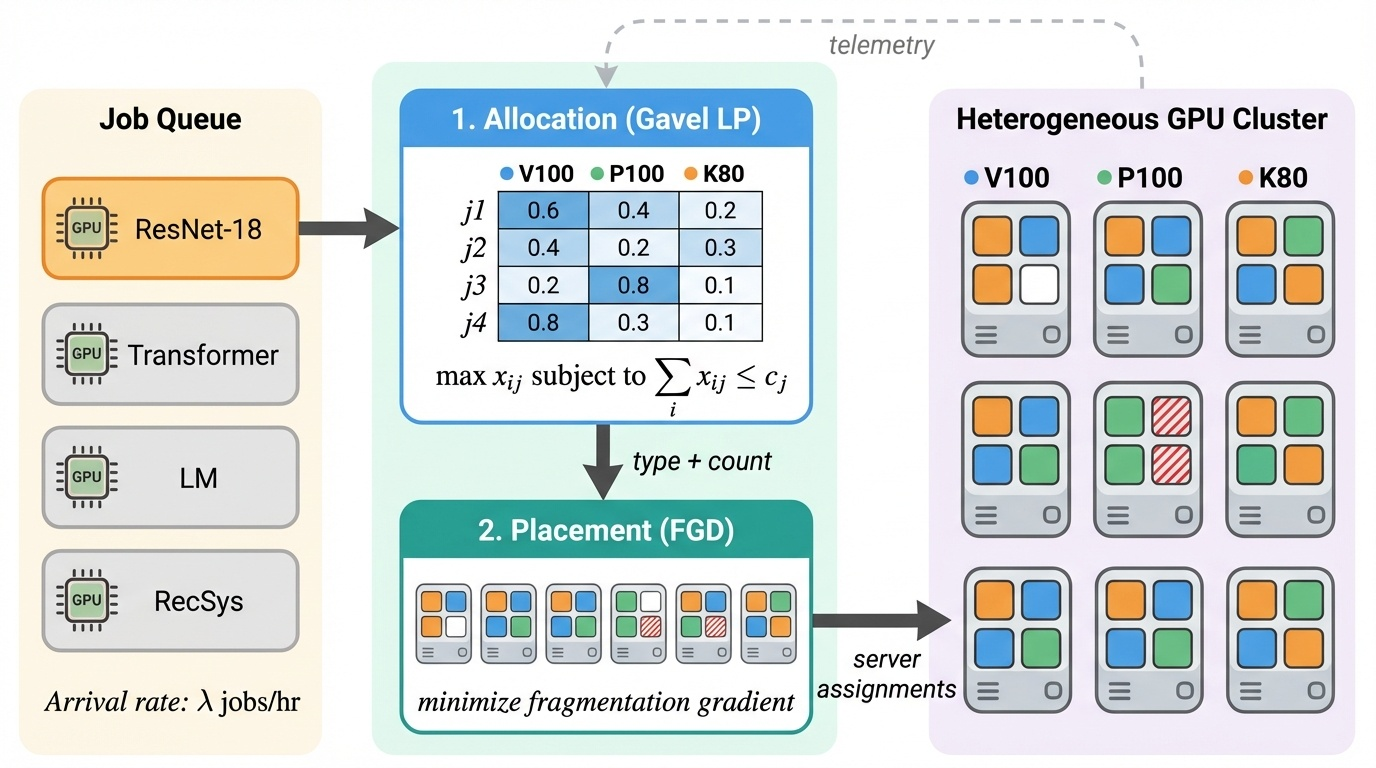
\includegraphics[width=\textwidth,height=0.42\textheight,keepaspectratio]{fig1_architecture.png}

  \vspace{2pt}

  \begin{columns}[T]
  \begin{column}{0.48\textwidth}
    \footnotesize\textbf{Stage 1 (Gavel):}\\
    LP allocates across GPU types.\\
    \textit{``Which type?''}
  \end{column}
  \begin{column}{0.48\textwidth}
    \footnotesize\textbf{Stage 2 (FGD):}\\
    Minimizes fragmentation gradient.\\
    \textit{``Which node?''}
  \end{column}
  \end{columns}
\end{column}
\end{columns}

\note{
  \begin{itemize}
    \item Left: research lineage -- two independent lines converge in our work.
    \item Right: two-stage architecture. Stage 1 picks GPU type, Stage 2 picks node.
    \item Clean separation -- allocation and placement are orthogonal.
    \item Also explored GavelFGD+: feeding placement availability back into LP.
    \item TRANSITION: How do we evaluate a combined system bridging two different methodologies?
  \end{itemize}
}

\end{frame}

% ============================================================
% SLIDE 4: Evaluation Methodology
% ============================================================
\begin{frame}{Evaluation: Replicate, Then Extend}

\begin{columns}[T]
\begin{column}{0.48\textwidth}
  \centering
  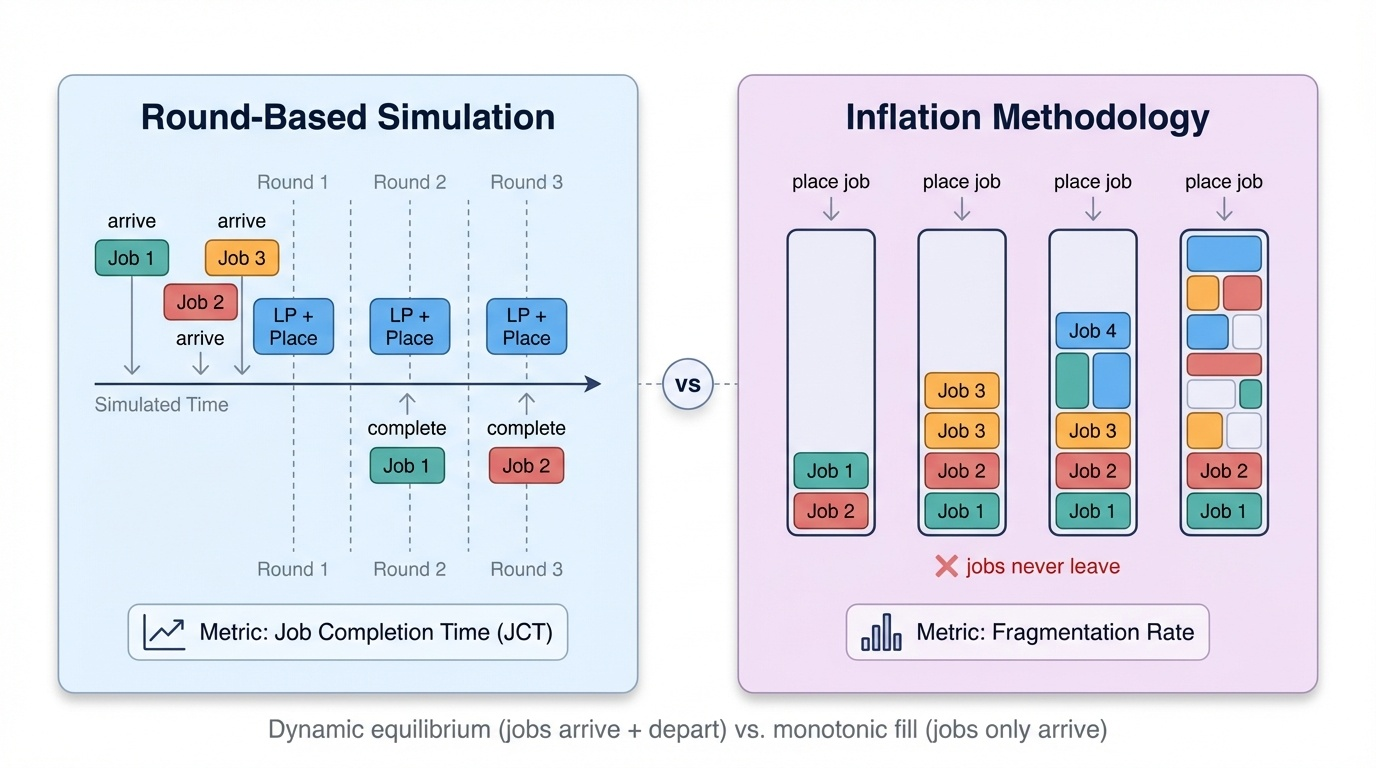
\includegraphics[width=\textwidth,height=0.45\textheight,keepaspectratio]{fig4_eval_methodology.png}\\[3pt]
  \footnotesize Gavel uses \textbf{round-based simulation} (dynamic arrivals, measures JCT).
  FGD uses \textbf{inflation methodology} (monotonic fill, measures fragmentation).
  We bridge both.
\end{column}
\begin{column}{0.48\textwidth}

\small\textbf{Phase 1: Replicate to validate}\\[1pt]
\footnotesize Gavel on Philly (504 exps) + FGD on Alibaba

\smallskip

\small\textbf{Phase 2--3: Extend with integration}\\[1pt]
\footnotesize Combined Gavel+FGD on 2 cluster topologies\\
15 rates $\times$ 3 seeds $\times$ 4 placements $\times$ 2 policies

\smallskip

\statbox{900 total experiments}

\smallskip

\footnotesize\textbf{Key variable:} node topology\\
Alibaba Split: \textbf{uniform} 8-GPU nodes\\
Cluster H: \textbf{mixed} 1/2/4/8-GPU nodes

\end{column}
\end{columns}

\note{
  \begin{itemize}
    \item Key challenge: Gavel and FGD use completely different evaluation methodologies.
    \item We first replicate each independently to validate our implementations.
    \item Then extend: combined system on two Alibaba cluster topologies.
    \item The two clusters isolate one variable: node size diversity.
    \item TRANSITION: Let's see the replication results...
  \end{itemize}
}

\end{frame}

% ============================================================
% SLIDE 5: Replication Validates Both Baselines
% ============================================================
\begin{frame}{Replication Validates Both Baselines}

\begin{columns}[T]
\begin{column}{0.48\textwidth}
  \centering
  \small\textbf{Gavel} (504 experiments, Philly trace)\\[2pt]
  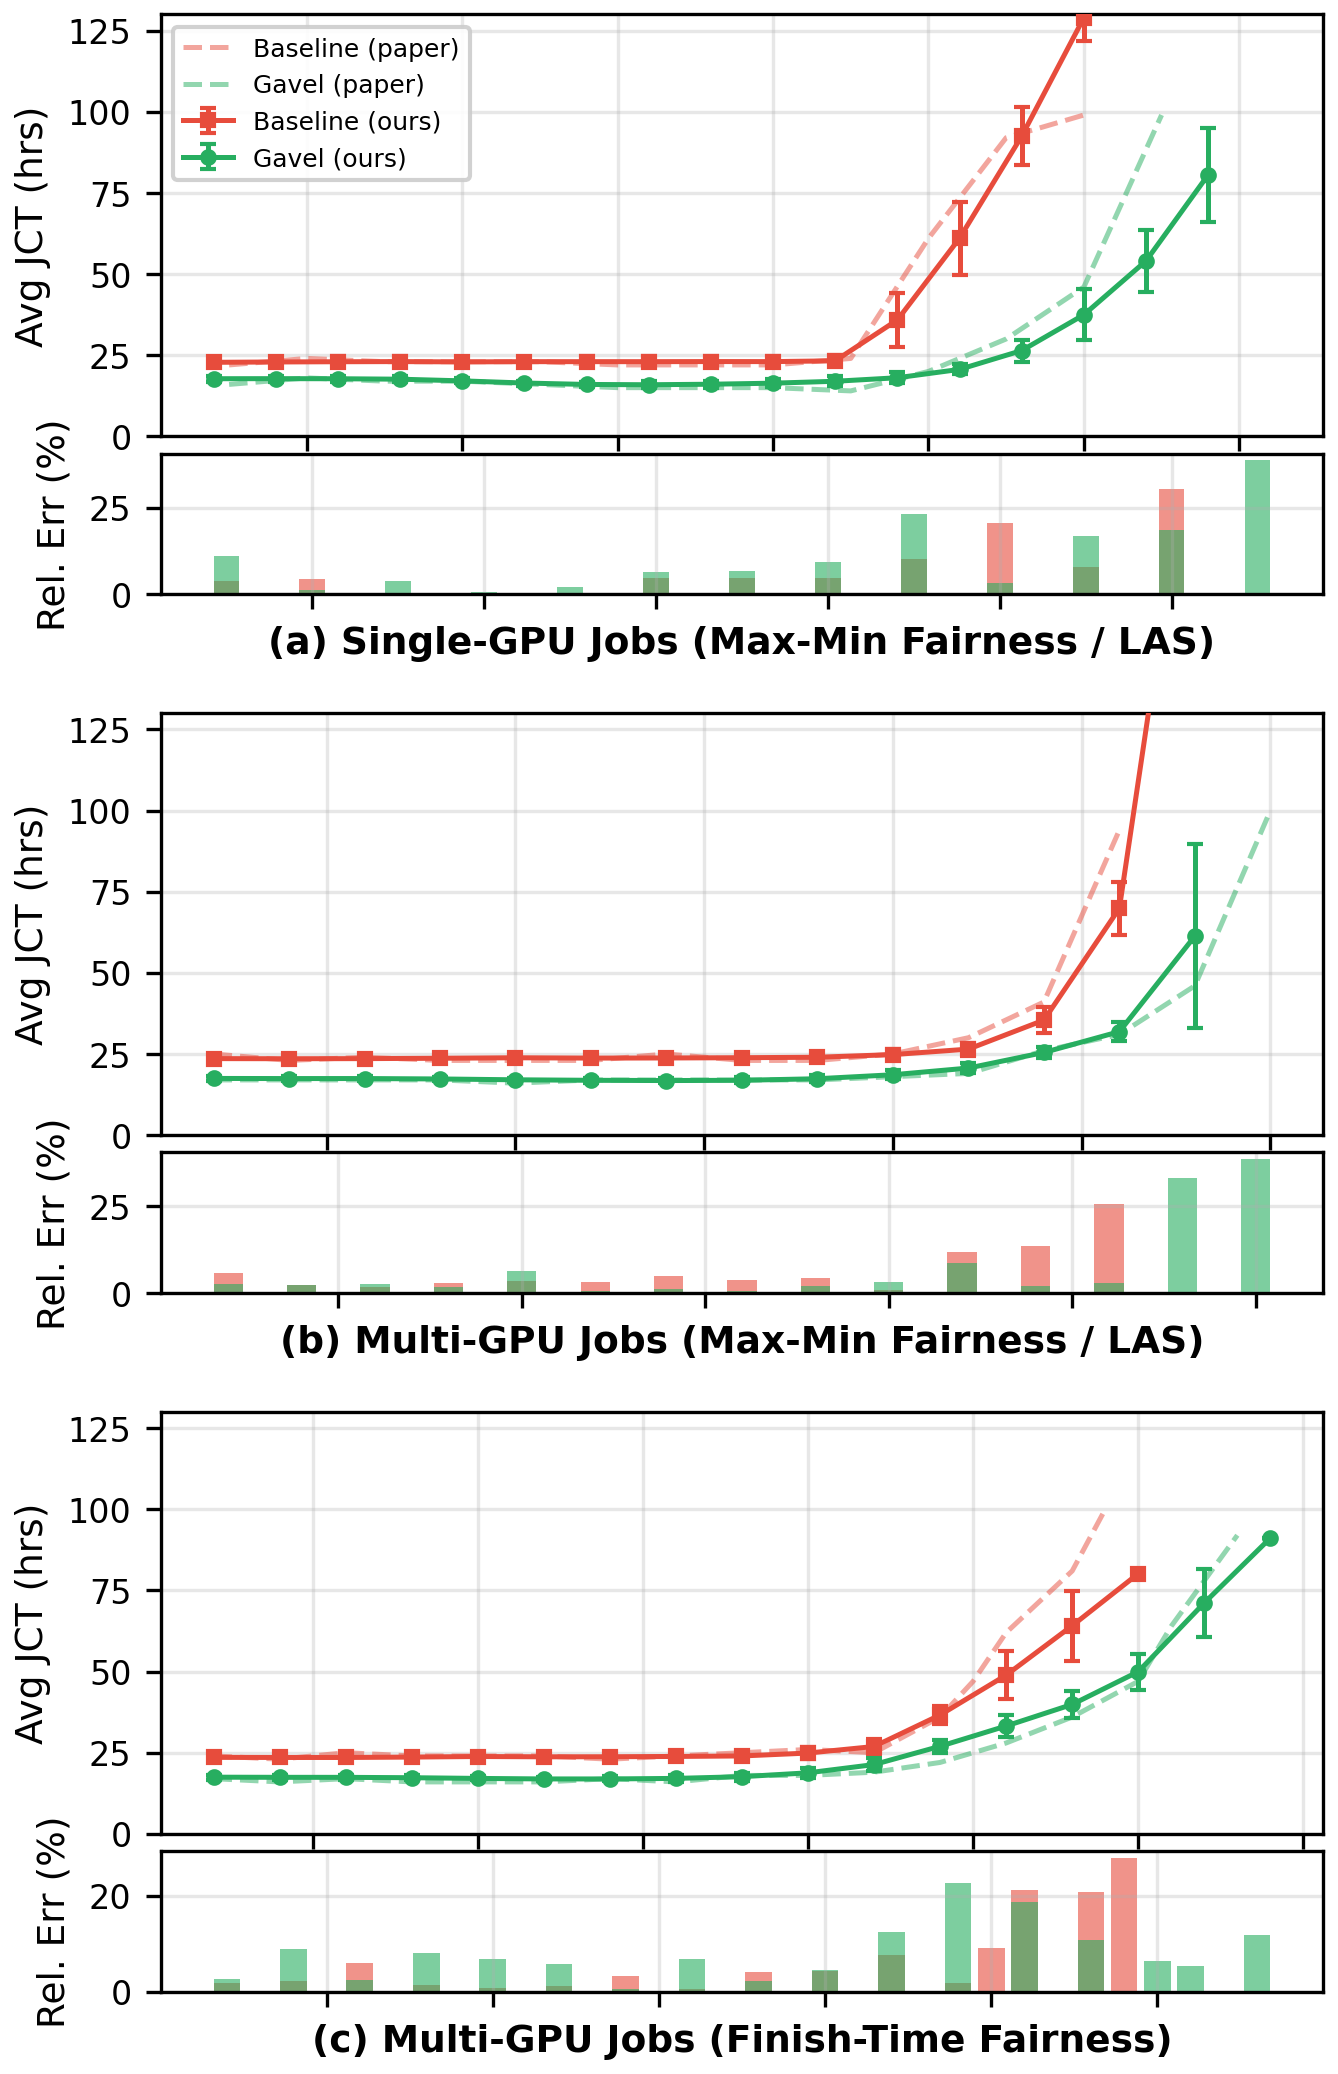
\includegraphics[width=\textwidth,height=0.65\textheight,keepaspectratio]{fig_gavel_replication.png}\\[1pt]
  \footnotesize Solid: ours. Dashed: paper reference.\\
  Close match at sub-saturation loads.
\end{column}
\begin{column}{0.48\textwidth}
  \centering
  \small\textbf{FGD} (Alibaba Cluster H, 6 policies)\\[2pt]
  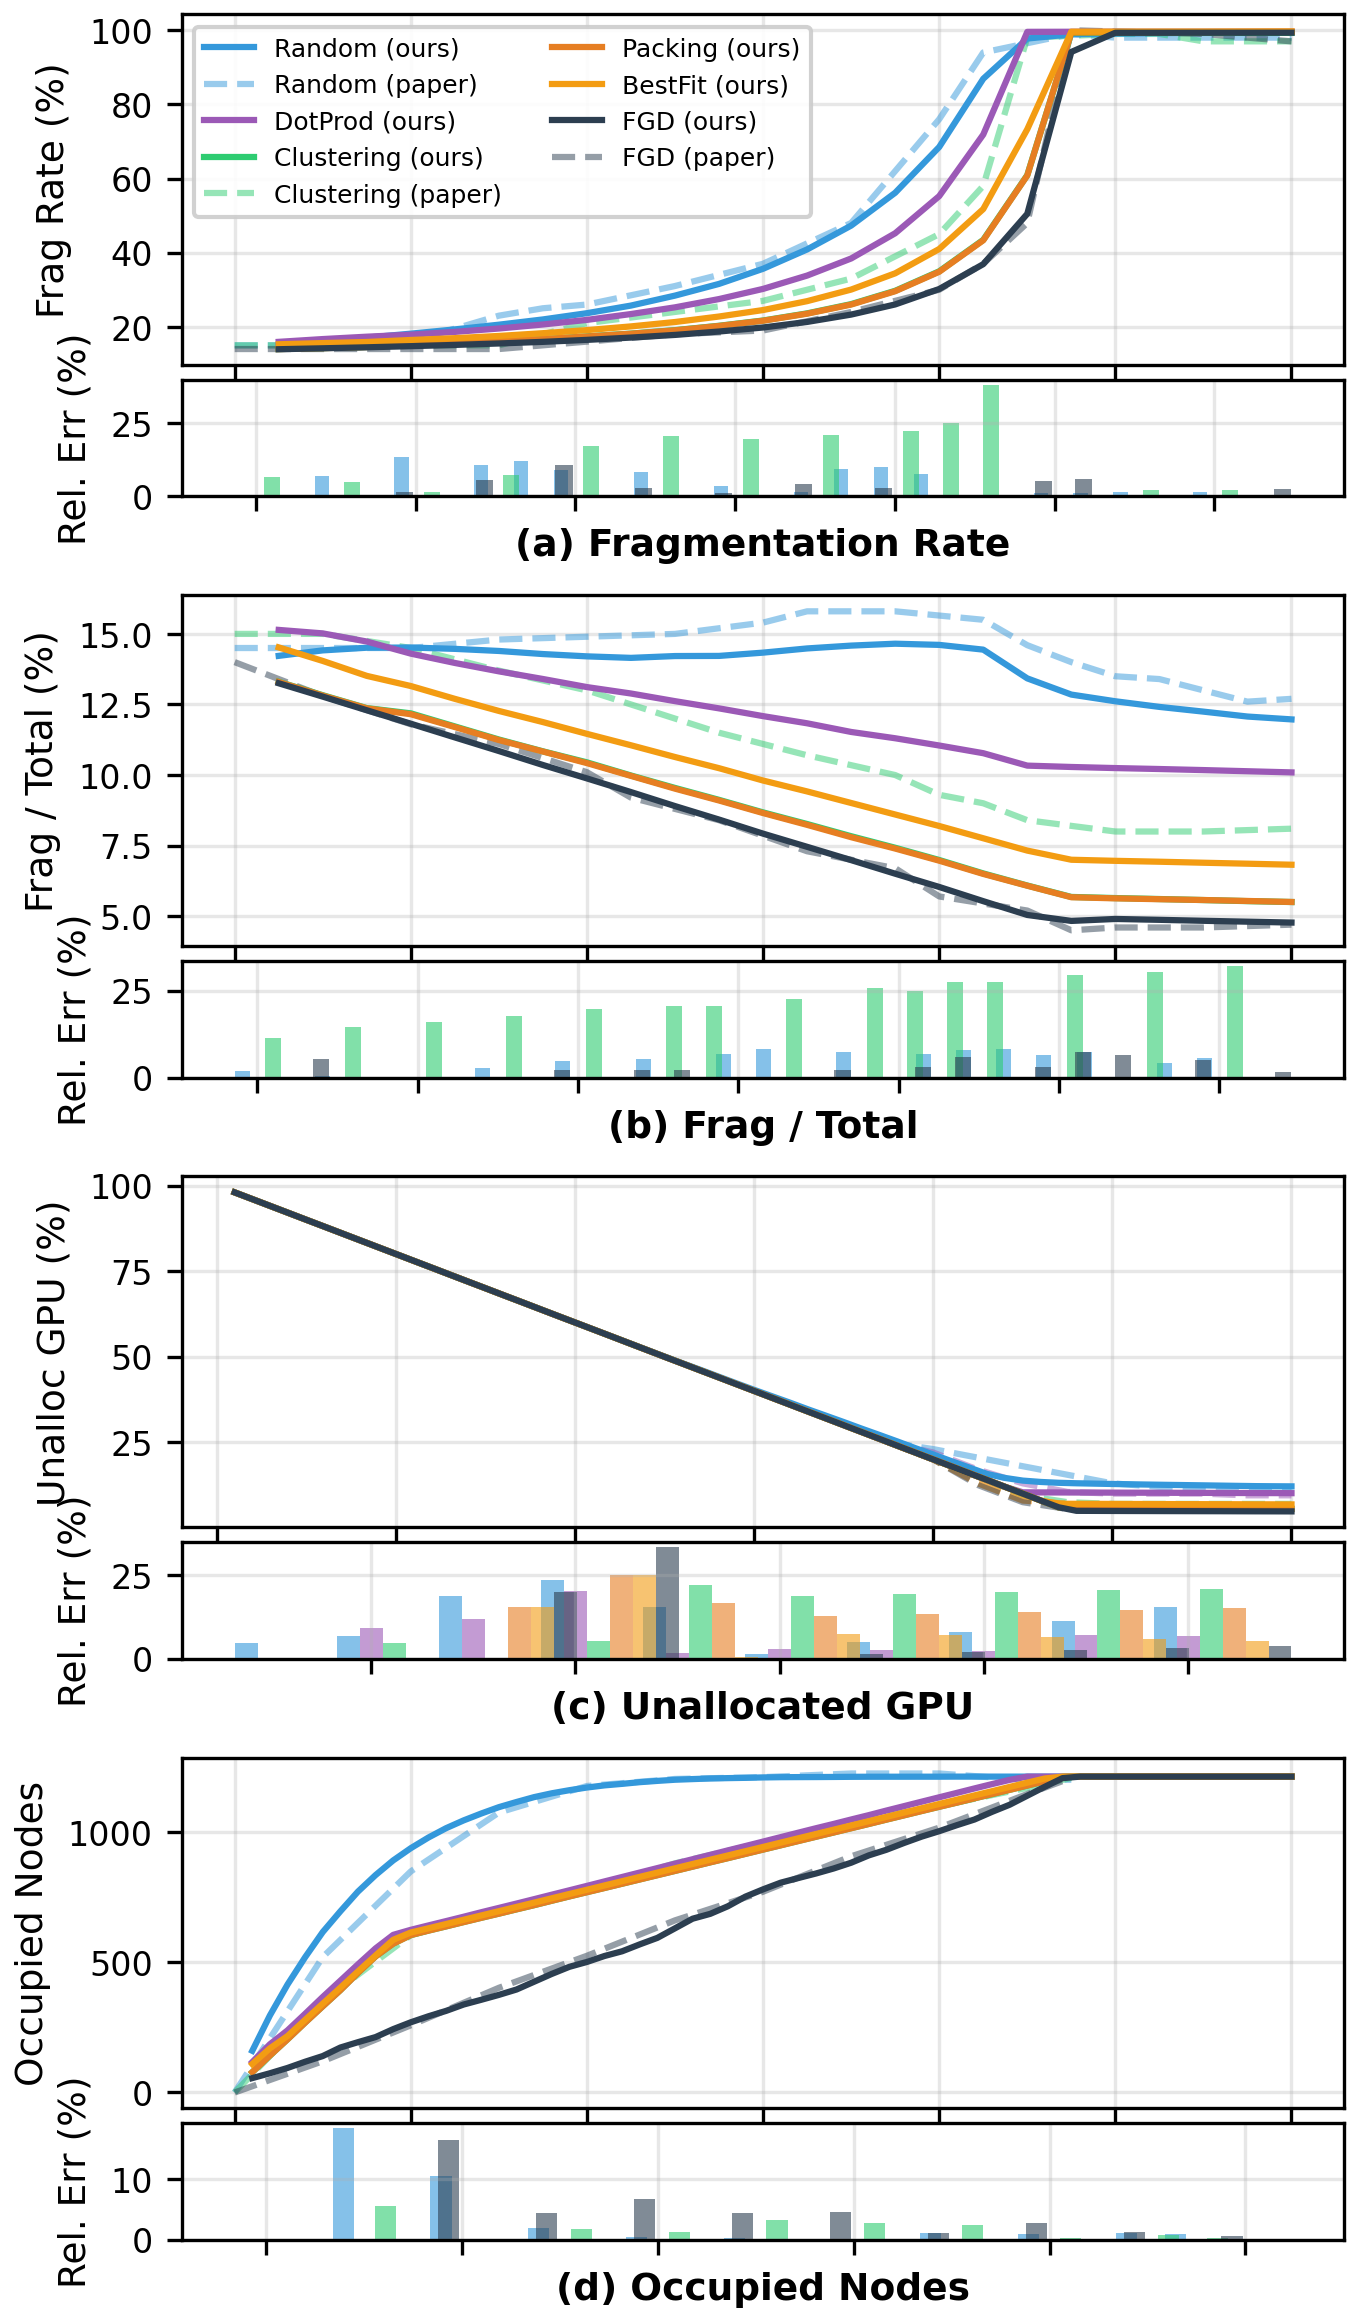
\includegraphics[width=\textwidth,height=0.65\textheight,keepaspectratio]{fig_fgd_replication.png}\\[1pt]
  \footnotesize At 80\% demand: Random fragments 85\%\\of free GPUs vs. FGD's 42\%.
\end{column}
\end{columns}

\note{
  \begin{itemize}
    \item Before combining, we replicated each system independently.
    \item Gavel: 504 experiments on Philly trace. Close match; divergence only near saturation.
    \item FGD: Cluster H, 6 placement policies. FGD maintains lowest fragmentation.
    \item This gives us confidence the integration compares real implementations, not artifacts.
    \item TRANSITION: Now the combined system results...
  \end{itemize}
}

\end{frame}

% ============================================================
% SLIDE 6: FGD Cuts Fragmentation 30-40% on Mixed Nodes
% ============================================================
\begin{frame}{FGD Reduces Fragmentation 30--40\% on Mixed Nodes}

\begin{columns}[T]
\begin{column}{0.50\textwidth}
  \centering
  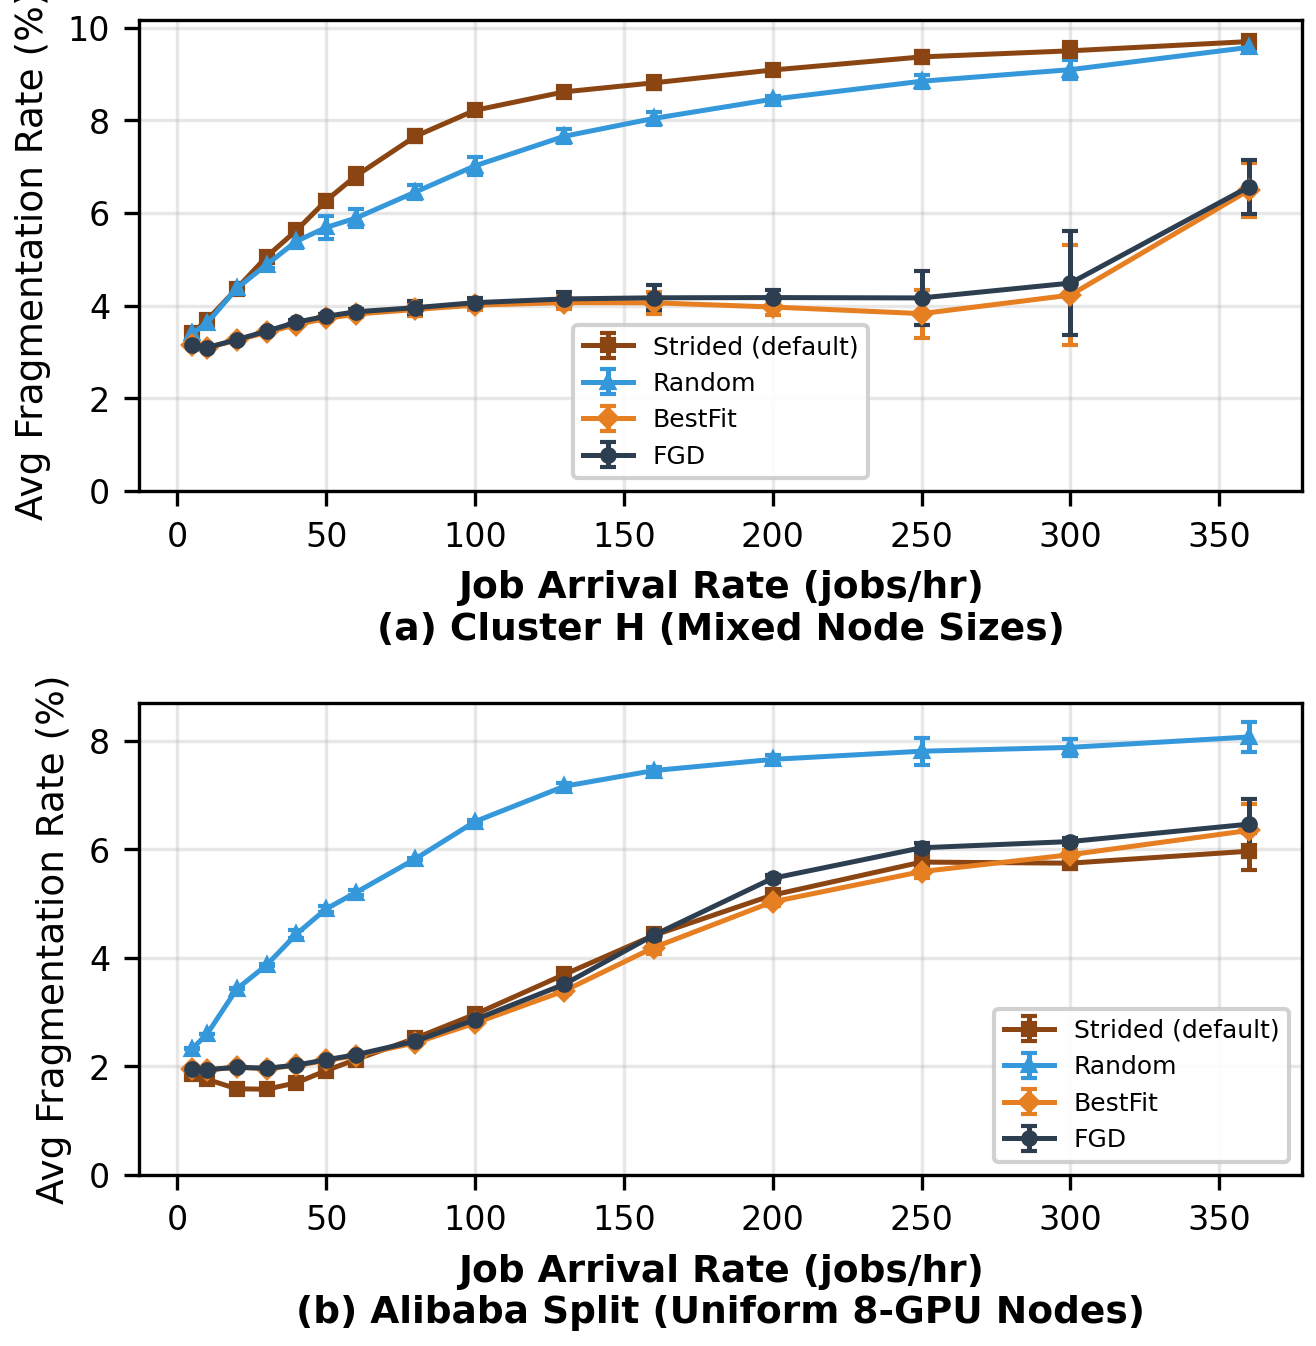
\includegraphics[width=\textwidth,height=0.7\textheight,keepaspectratio]{fig_jct_comparison.png}
\end{column}
\begin{column}{0.46\textwidth}

\textbf{Cluster H} (mixed 1/2/4/8-GPU nodes)

\medskip

FGD and BestFit reduce fragmentation by \textbf{40--50\%} vs. Strided across all arrival rates.

\medskip

Consistent ordering:\\
FGD $\approx$ BestFit $<$ Random $<$ Strided

\medskip

Holds under \textbf{both} Max-Min Fairness and FIFO.

\medskip

\small\textit{Placement benefit is independent of allocation policy.}

\end{column}
\end{columns}

\note{
  \begin{itemize}
    \item On Cluster H, FGD and BestFit reduce fragmentation by 40-50\% vs. Strided.
    \item Ordering is consistent across the full arrival rate sweep.
    \item This holds under both MMF and FIFO -- placement benefit is policy-independent.
    \item So far, exactly what we'd expect. FGD works.
    \item TRANSITION: But then we ran the same experiment on uniform nodes...
  \end{itemize}
}

\end{frame}

% ============================================================
% SLIDE 7: Zero Benefit on Uniform Nodes (The Twist)
% ============================================================
\begin{frame}{But Zero Benefit on Uniform Nodes}

\begin{columns}[T]
\begin{column}{0.38\textwidth}
  \centering
  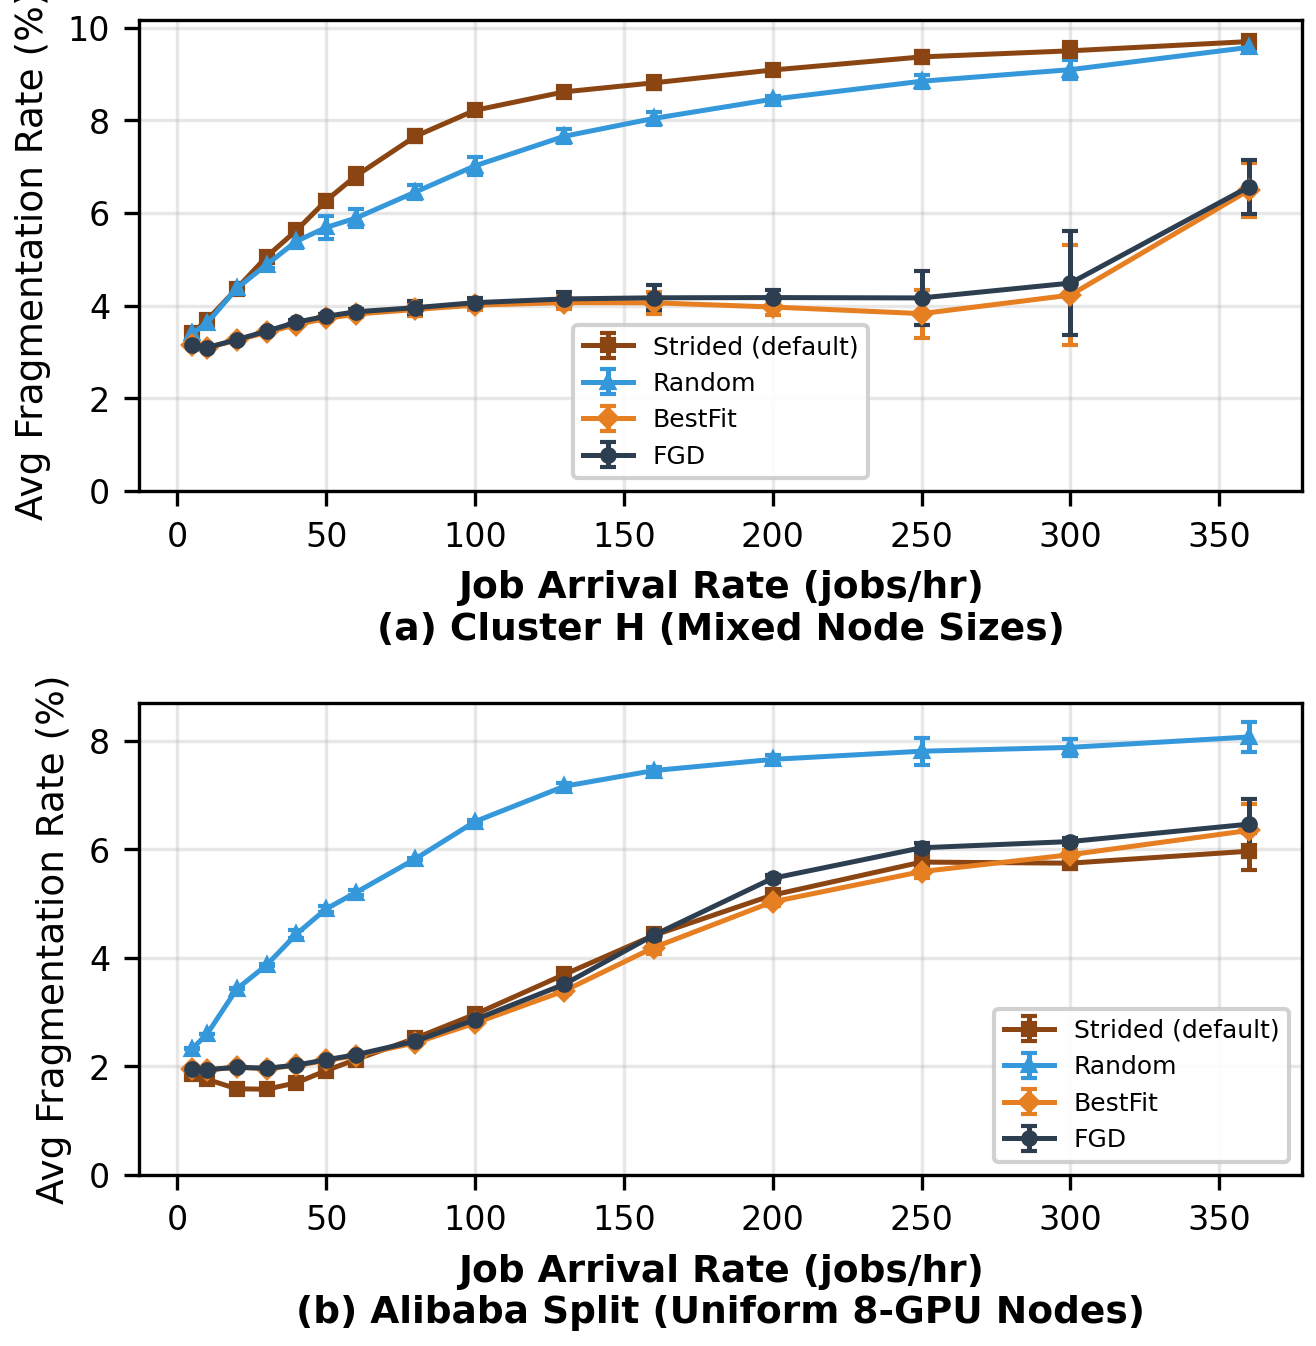
\includegraphics[width=\textwidth,height=0.62\textheight,keepaspectratio]{fig_jct_comparison.png}\\[2pt]
  \footnotesize (a) Mixed nodes: curves spread\\(b) Uniform nodes: curves converge
\end{column}
\begin{column}{0.58\textwidth}
  \centering
  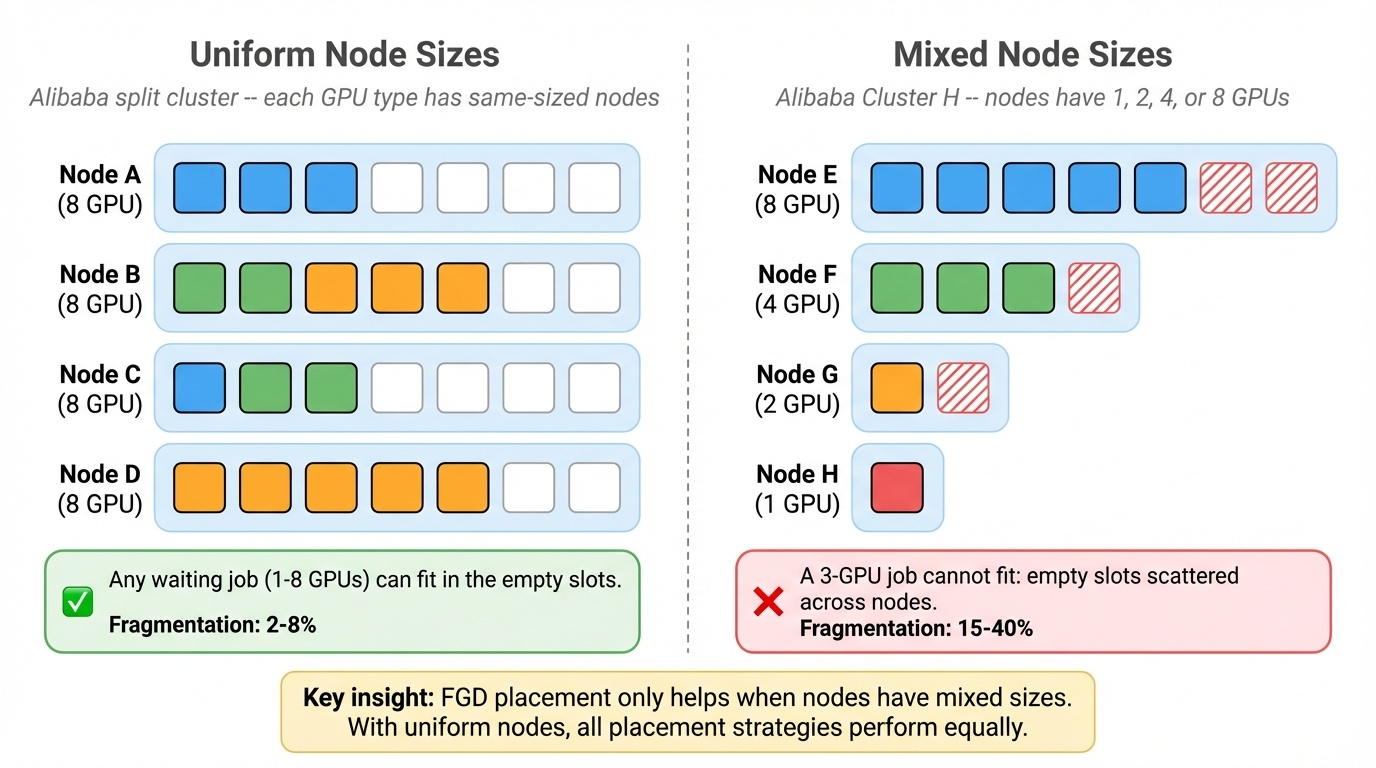
\includegraphics[width=0.9\textwidth,height=0.38\textheight,keepaspectratio]{fig2_topology.png}

  \vspace{4pt}

  \insightbox{Fragmentation depends on \textit{node topology diversity},\\ not GPU type heterogeneity.}
\end{column}
\end{columns}

\note{
  \begin{itemize}
    \item Same simulator, traces, placement algorithms. Only difference: node topology.
    \item On uniform 8-GPU nodes, ALL four strategies produce identical fragmentation.
    \item Why? Any job that fits on one node fits equally well on any other.
    \item On mixed nodes, a 3-GPU job can't use scattered 1-GPU fragments -- placement matters.
    \item CENTRAL FINDING. Pause here to let it land.
    \item TRANSITION: And this has real capacity implications...
  \end{itemize}
}

\end{frame}

% ============================================================
% SLIDE 8: Practical Impact
% ============================================================
\begin{frame}{Practical Impact: 280 GPUs Recovered}

\begin{columns}[T]
\begin{column}{0.52\textwidth}
  \centering
  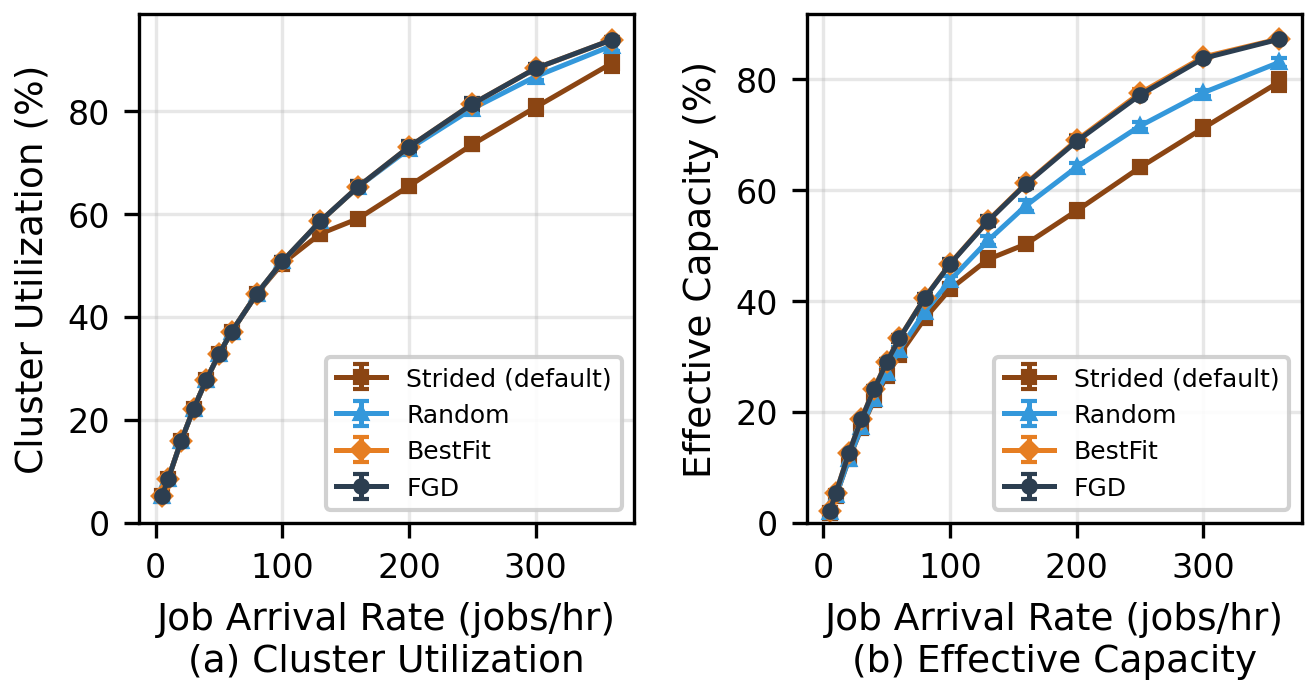
\includegraphics[width=\textwidth,height=0.72\textheight,keepaspectratio]{fig_utilization_impact.png}
\end{column}
\begin{column}{0.45\textwidth}

\small On Cluster H (mixed nodes):

\medskip

\statbox{280 recoverable GPUs}

\smallskip

\statbox{17\% more completed jobs}

\medskip

\begin{itemize}\small
  \item Strided caps at 89\% utilization
  \item FGD reaches 94\%
  \item Effective capacity gap: \textbf{13 points} at high load
\end{itemize}

\medskip

\footnotesize \textit{Per-job JCT identical across placements.\\
Placement shapes capacity; allocation shapes throughput.}

\end{column}
\end{columns}

\note{
  \begin{itemize}
    \item On mixed-node Cluster H, the fragmentation gap translates directly to usable capacity.
    \item Strided leaves 280 GPUs of fragmented, unusable capacity.
    \item Effective capacity gap of 13 points = 17\% more jobs completed.
    \item Per-job completion time is identical -- placement and allocation are orthogonal.
    \item TRANSITION: A few honest caveats, then a tool we built...
  \end{itemize}
}

\end{frame}

% ============================================================
% SLIDE 9: Limitations + Viz Tool
% ============================================================
\begin{frame}{Limitations \& Visualization Tool}

\begin{columns}[T]
\begin{column}{0.48\textwidth}

\textbf{Honest caveats:}

\begin{itemize}
  \item FGD is \textbf{sensitive to workload ordering} -- underperforms in 5/7 arrival orders
  \item All results are \textbf{trace-driven simulation} -- no feedback effects
  \item \textbf{Migration costs} not modeled
\end{itemize}

\end{column}
\begin{column}{0.48\textwidth}

\textbf{Interactive Visualization Tool:}

\smallskip

\href{https://youtu.be/Z24wVt0xIxk}{%
\begin{tikzpicture}
  \node[inner sep=0] (img) {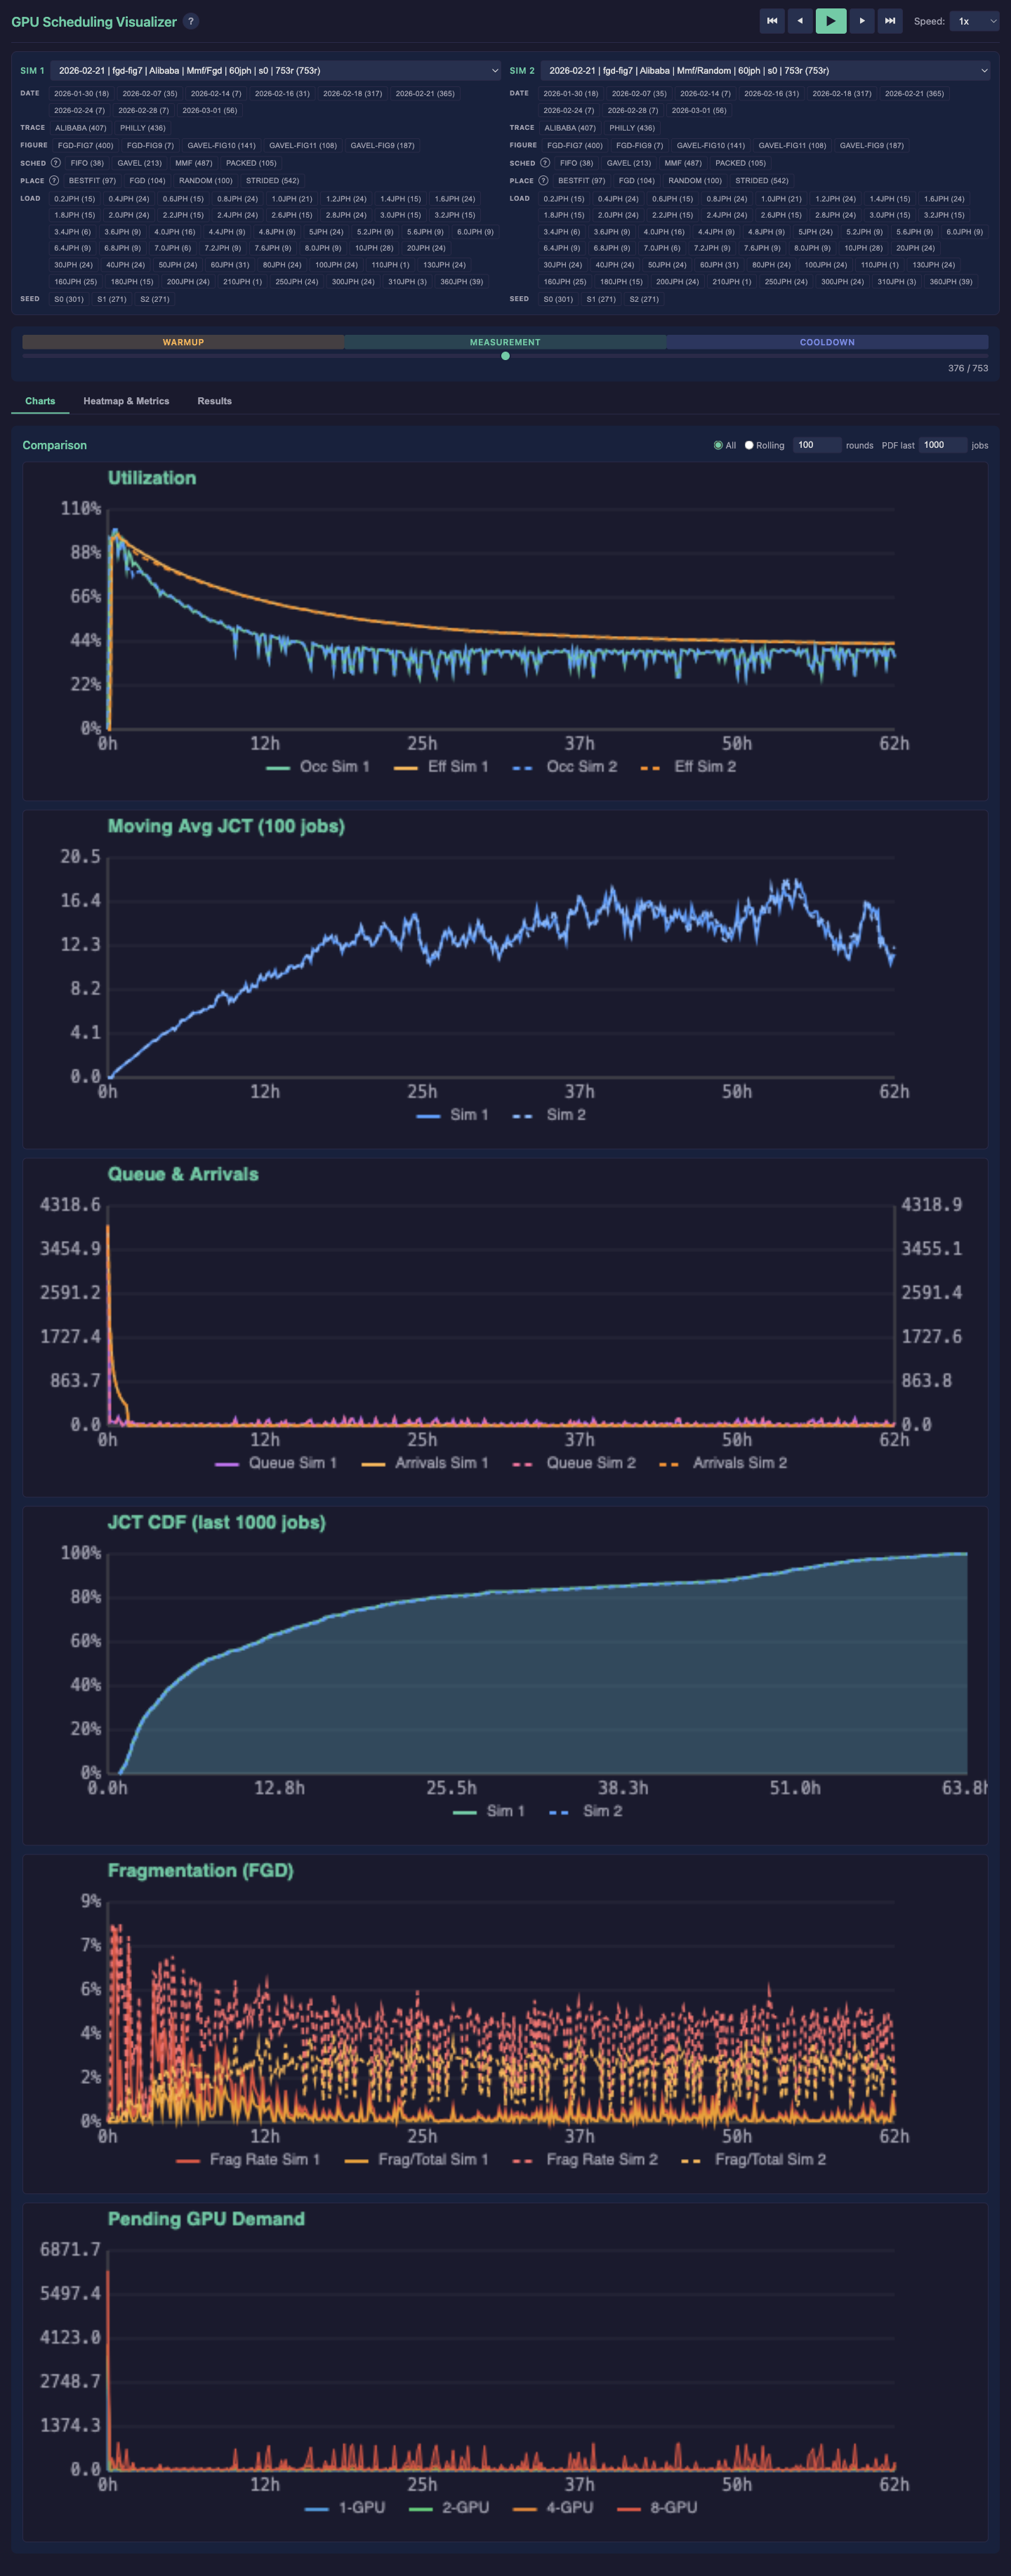
\includegraphics[width=\textwidth,height=0.45\textheight,keepaspectratio]{fig_viz_timeseries.png}};
  \node[fill=cardinalred, text=white, rounded corners=3pt, inner sep=4pt, font=\footnotesize\bfseries] at (img.south) {$\blacktriangleright$\ Click to Play Demo};
\end{tikzpicture}}

\smallskip

\footnotesize 843 experiments. Side-by-side comparison, time-series charts, aggregate results. \href{https://youtu.be/Z24wVt0xIxk}{\textcolor{darkcyan}{\underline{Demo video}}}

\end{column}
\end{columns}

\note{
  \begin{itemize}
    \item FGD sensitive to arrival order -- wins only when large jobs arrive first.
    \item Trace-driven simulation has no feedback effects, no real migration costs.
    \item [Play demo clip] Built interactive viz tool to explore all 843 experiments.
    \item [If time: switch to live tab for quick walkthrough]
    \item TRANSITION: So what should you take away?
  \end{itemize}
}

\end{frame}

% ============================================================
% SLIDE 10: Takeaway
% ============================================================
\begin{frame}{}

\vfill

\begin{center}

{\Large \textbf{Fragmentation is driven by \textit{node topology diversity},\\[6pt] not GPU type heterogeneity.}}

\vspace{24pt}

\begin{columns}[T]
\begin{column}{0.8\textwidth}
\begin{enumerate}
  \item \textbf{Uniform clusters} don't need fragmentation-aware placement
  \item \textbf{Mixed-hardware clusters} benefit substantially (30--40\% less fragmentation, 17\% more throughput)
  \item \textbf{Allocation and placement are orthogonal} -- compose them independently
\end{enumerate}
\end{column}
\end{columns}

\vspace{18pt}

\small
Simulator: \texttt{github.com/Turquoise-T/cs244c-GPU\_fragment}\\
Viz tool: \texttt{github.com/varunr89/gpu-scheduling-viz}

\end{center}

\vfill

\note{
  \begin{itemize}
    \item New uniform clusters don't need fragmentation-aware placement.
    \item Clusters with accumulated mixed hardware benefit substantially.
    \item Allocation and placement are orthogonal -- you can compose them independently.
    \item Code is open source.
    \item END. Open for questions.
  \end{itemize}
}

\end{frame}

% ============================================================
% BACKUP SLIDES
% ============================================================
\appendix

\begin{frame}{Backup: Arrival Order Sensitivity}

\begin{center}
\small
\begin{tabular}{lccc}
\toprule
\textbf{Task arrival order} & \textbf{FGD} & \textbf{Clustering} & \textbf{Random} \\
\midrule
trace          & 480.0  & 205.5  & 522.0  \\
ascending      & 2167.0 & 835.0  & 1029.0 \\
descending     & 110.2  & 129.0  & 107.6  \\
phased 01234   & 1890.0 & 808.0  & 993.0  \\
phased 12034   & 1318.0 & 332.0  & 925.0  \\
phased 24031   & 949.0  & 162.0  & 586.0  \\
phased 31042   & 124.0  & 267.9  & 421.7  \\
\bottomrule
\end{tabular}
\end{center}

\medskip

Total pending task GPUs at 96\% arrived workload (Alibaba, 90\% cluster scale).\\
FGD underperforms Clustering in 5 of 7 orderings. Wins only when large jobs arrive first.

\end{frame}

\begin{frame}{Backup: GavelFGD+ (POA Coordination)}
\begin{center}
  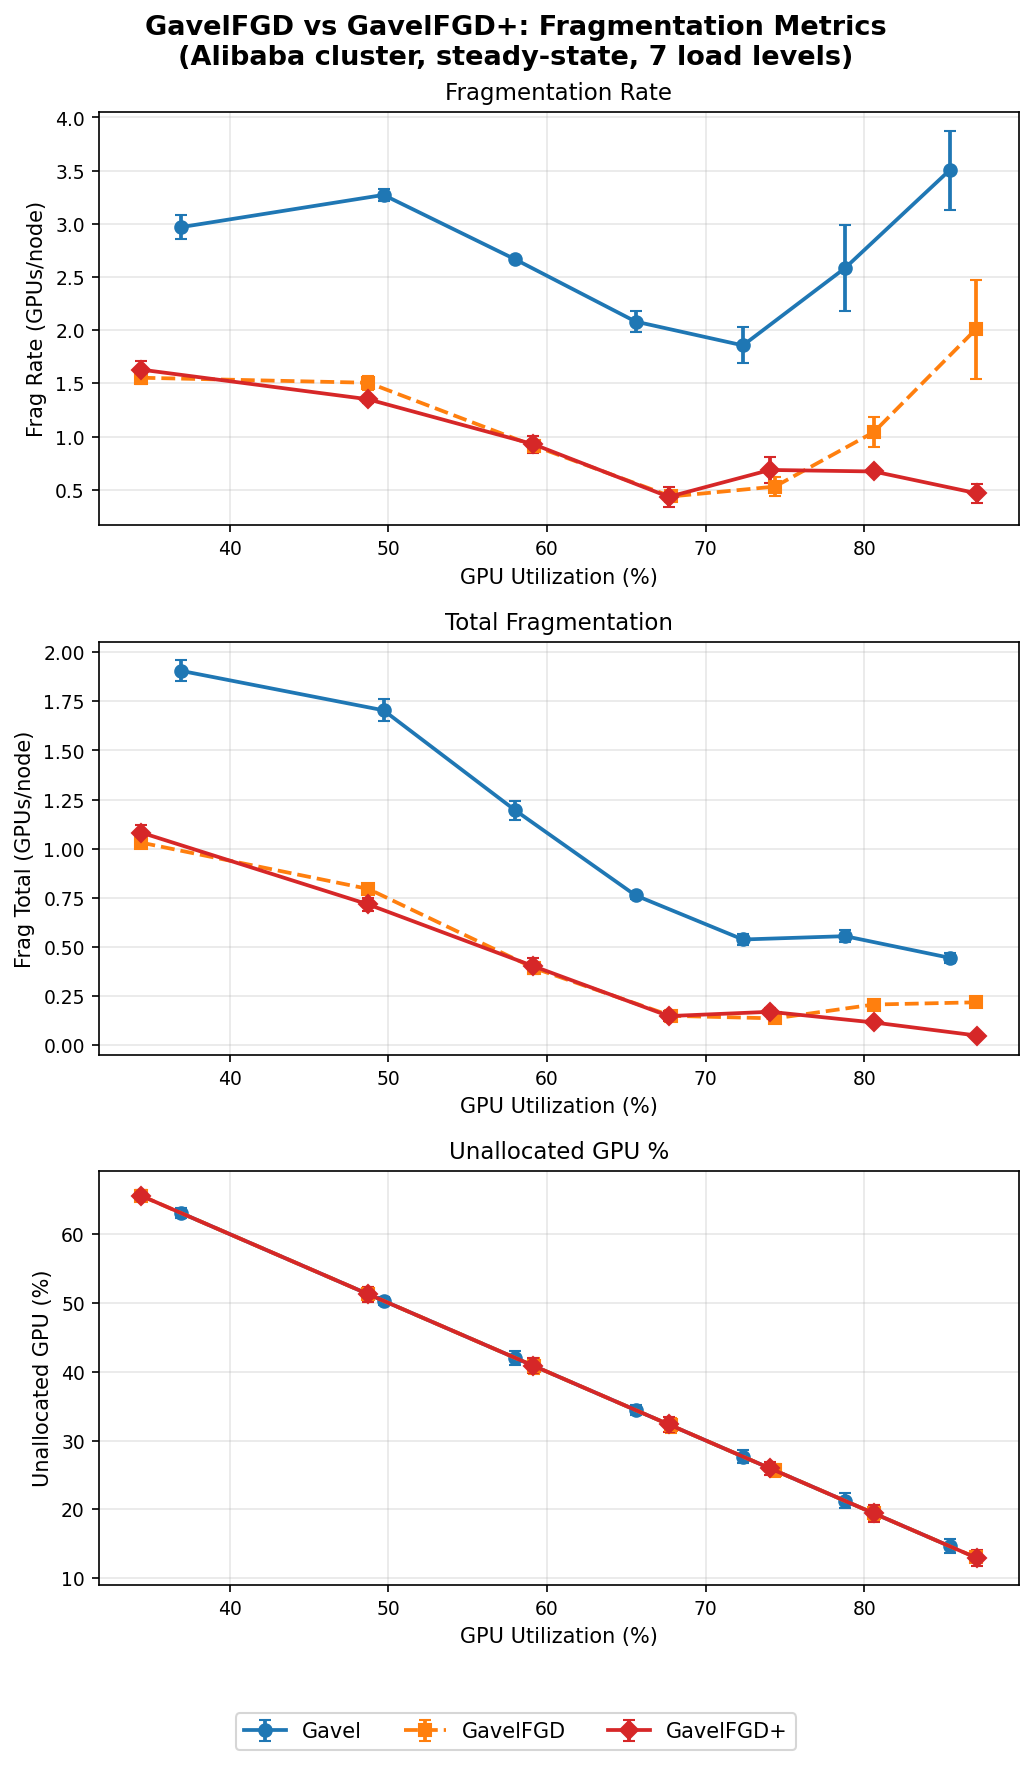
\includegraphics[width=0.45\textwidth,height=0.65\textheight,keepaspectratio]{gavelfgd_combined_absolute.png}
\end{center}
\small At 85\% utilization, GavelFGD+ reduces fragmentation by 76.7\% relative to GavelFGD.\\
Improvement comes from more efficient packing, not additional resources.
\end{frame}

\begin{frame}{Backup: Wall Time Analysis}
\begin{center}
  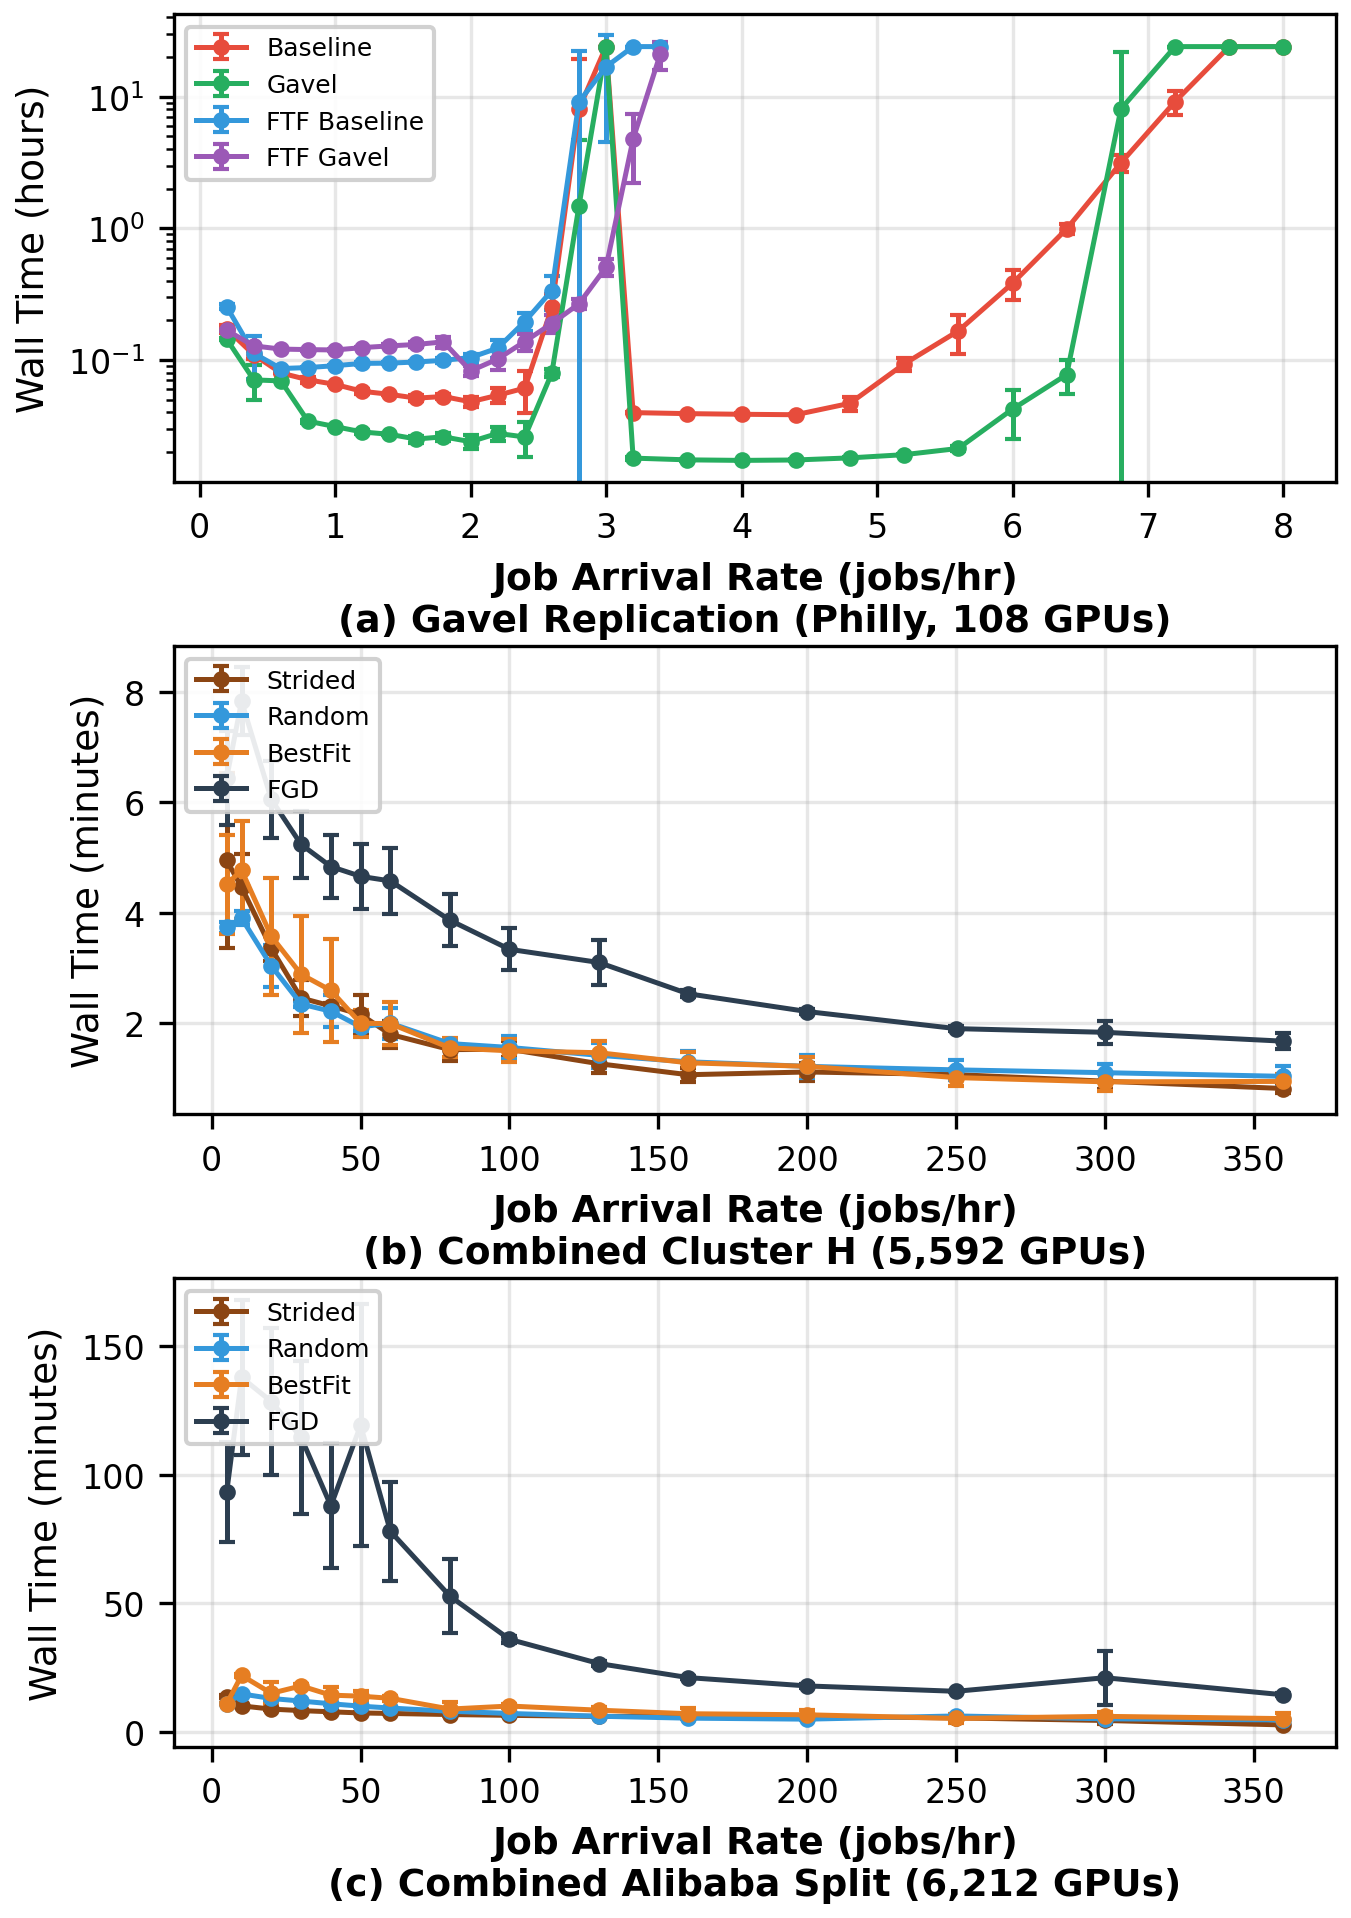
\includegraphics[width=0.40\textwidth,height=0.65\textheight,keepaspectratio]{fig_wall_time.png}
\end{center}
\small 900+ experiments on Stanford FarmShare (Intel Xeon, no GPU required).\\
Philly: exponential near saturation. Cluster H: flat 1--6 min. Alibaba: decreasing with load.
\end{frame}

\begin{frame}{Backup: Per-Utilization Cluster H}
\begin{center}
  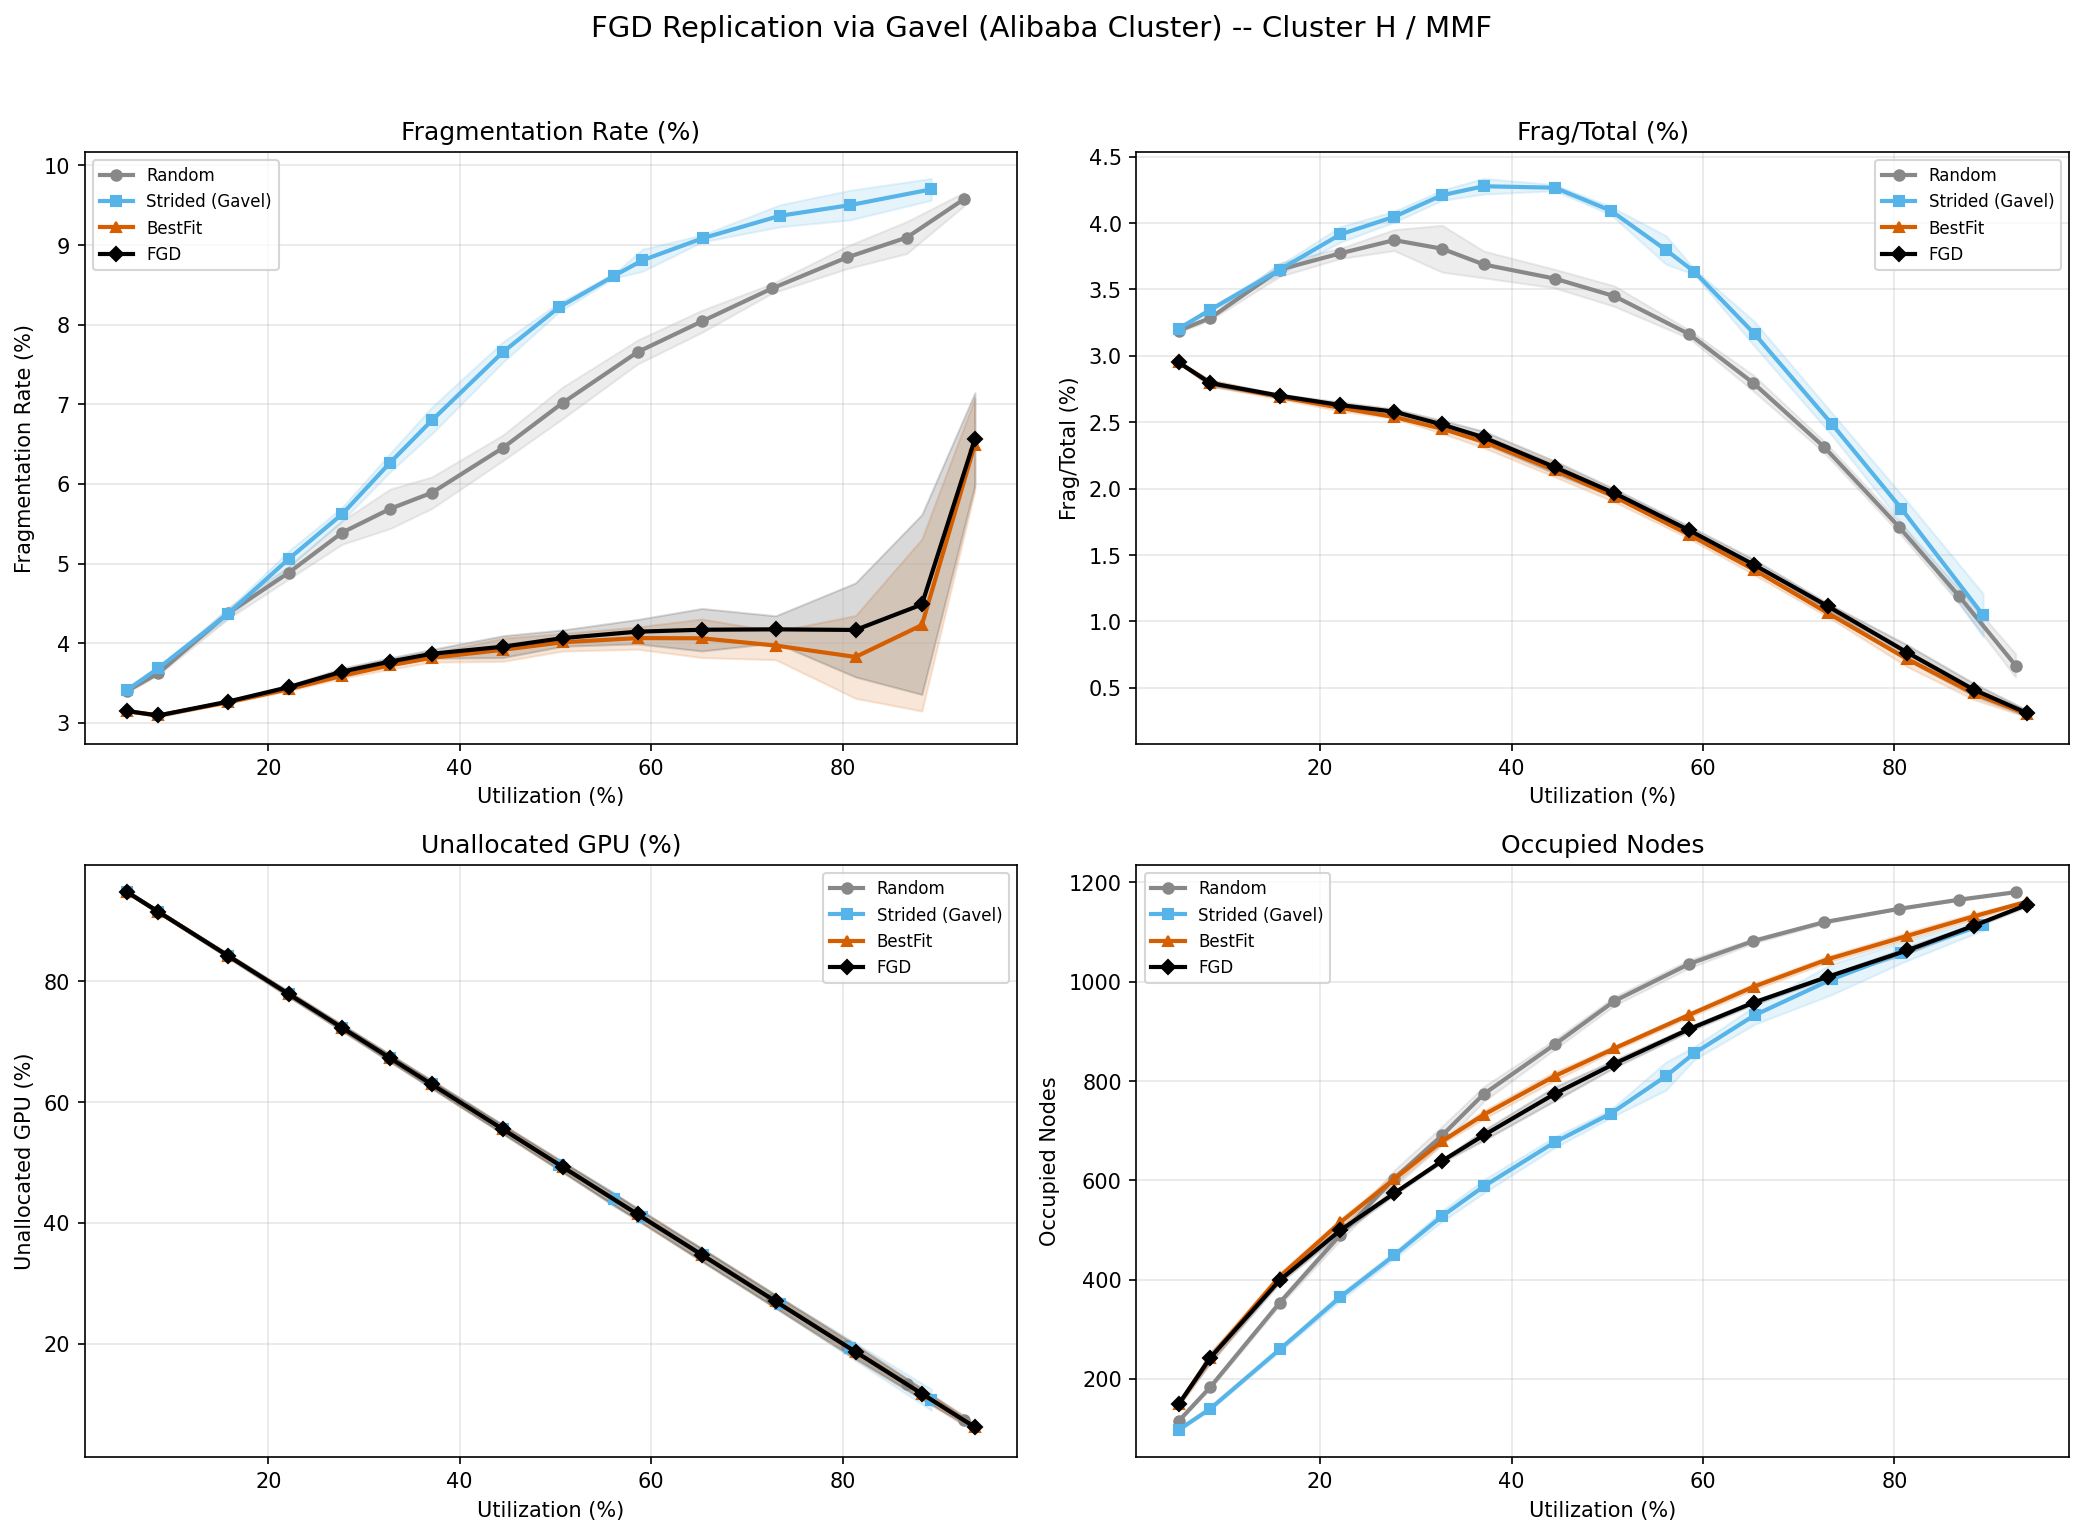
\includegraphics[width=0.55\textwidth,height=0.65\textheight,keepaspectratio]{fig7_combined_cluster_h.png}
\end{center}
\small FGD (black) reduces fragmentation by 30--40\% vs. Random (blue) at moderate utilization.\\
BestFit (orange) is intermediate. Strided (brown) tracks Random.
\end{frame}

\begin{frame}{Backup: Per-Utilization Alibaba Split (Uniform)}
\begin{center}
  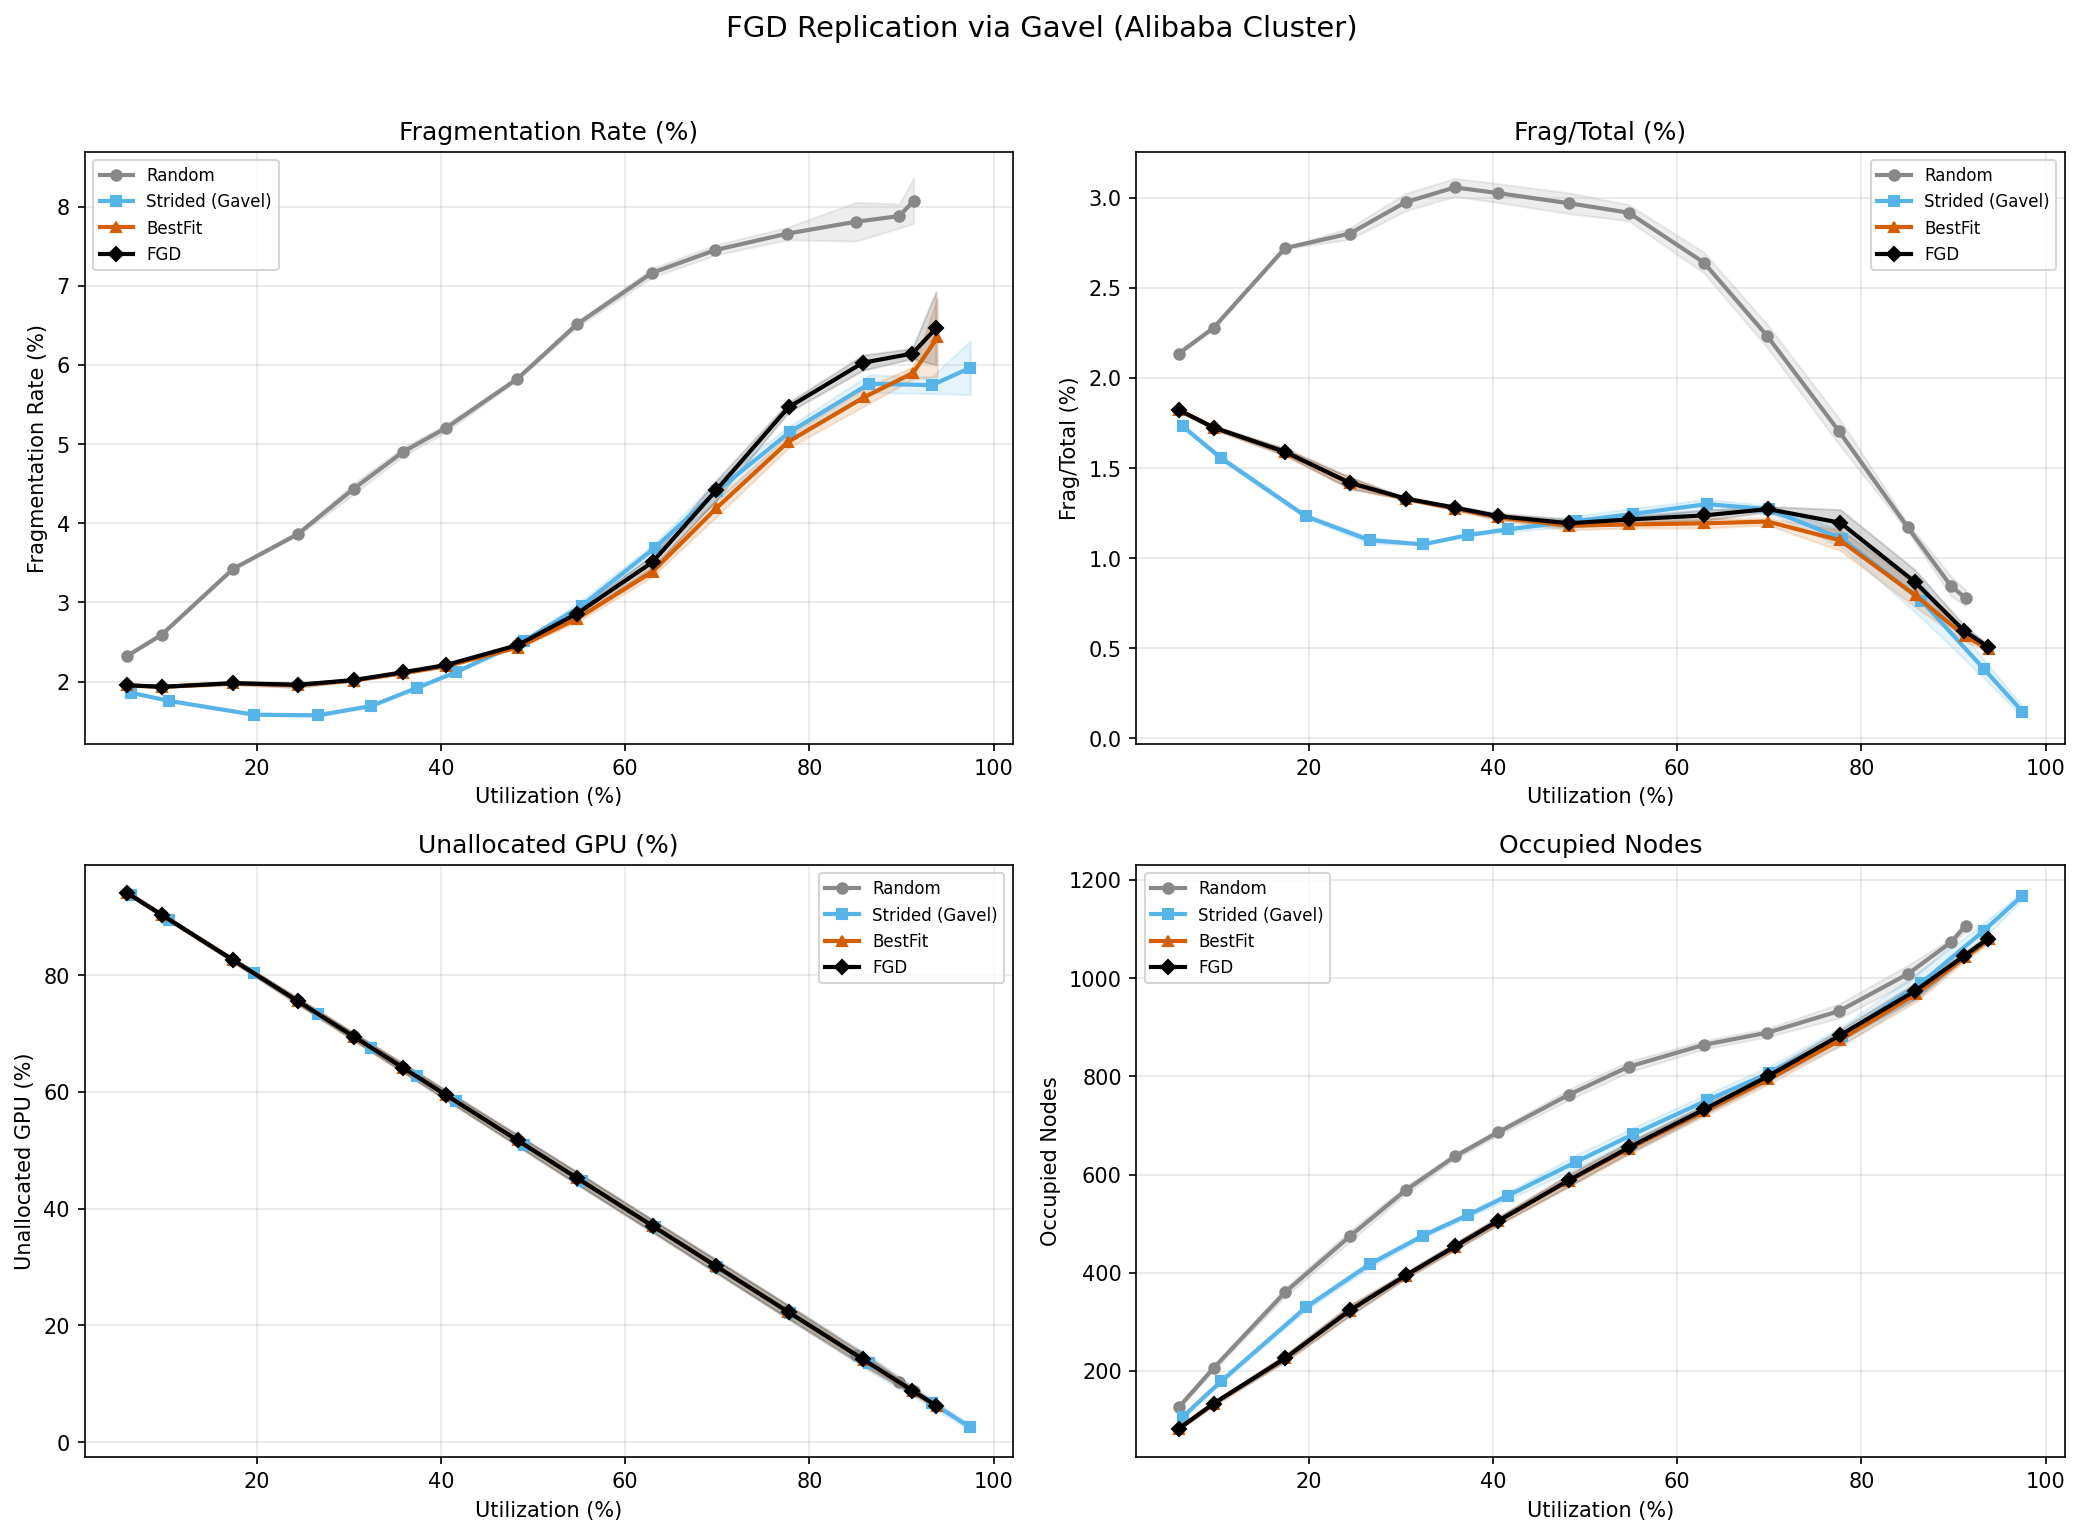
\includegraphics[width=0.55\textwidth,height=0.65\textheight,keepaspectratio]{fig8_combined_uniform.png}
\end{center}
\small All placement strategies converge. Node topology uniformity eliminates the fragmentation problem.
\end{frame}

\end{document}
